%!TEX program = xelatex
% ==============================================
% 广东工业大学 传感器技术与应用 调研报告
% 自动驾驶汽车先进传感器技术综述
% ==============================================
\documentclass[12pt,a4paper,openany,UTF8]{ctexbook}

% 字体设置
\setmainfont{Times New Roman}
\setsansfont{Times New Roman}
\setmonofont{Consolas}

% 页边距
\usepackage{geometry}
\geometry{top=30mm, bottom=25mm, left=30mm, right=20mm, includeheadfoot}

% 行距与缩进
\usepackage{setspace}
\onehalfspacing
\setlength{\parindent}{2em}
\setlength{\parskip}{0pt}

% 标题格式
\usepackage{titlesec}
\titleformat{\chapter}[block]
    {\centering\fontsize{16pt}{18pt}\selectfont\bfseries\heiti}
    {第\thechapter 章}{1em}{}
\titleformat{\section}[block]
    {\fontsize{12pt}{14pt}\selectfont\bfseries\heiti}
    {\thesection}{0.5em}{}
\titleformat{\subsection}[block]
    {\fontsize{12pt}{14pt}\selectfont\heiti}
    {\thesubsection}{0.5em}{}

% 页眉页脚
\usepackage{fancyhdr}
\pagestyle{fancy}
\fancyhf{}
\fancyfoot[R]{\fontsize{10.5pt}{12pt}\selectfont\thepage}
\renewcommand{\headrulewidth}{0pt}

% 宏包
\usepackage{amsmath}
\usepackage{graphicx}
\usepackage{booktabs}
\usepackage{enumitem}
\usepackage{longtable}
\usepackage{array}
\usepackage{multirow}
\usepackage{tikz}
\usetikzlibrary{shapes.geometric, arrows.meta, positioning, calc, backgrounds, fit}
\usepackage{xcolor}
\usepackage{colortbl}
\usepackage{gbt7714}
\bibliographystyle{gbt7714-numerical}

% 图表按章编号
\usepackage{chngcntr}
\counterwithin{figure}{chapter}
\counterwithin{table}{chapter}

% 代码
\usepackage{listings}
\usepackage{xcolor}
\lstset{
    basicstyle=\ttfamily\small,
    keywordstyle=\color{blue},
    commentstyle=\color{green!60!black},
    stringstyle=\color{red},
    breaklines=true,
    frame=single,
    numbers=left,
    numberstyle=\tiny\color{gray}
}

% 超链接
\usepackage[colorlinks=true,linkcolor=black,citecolor=blue,urlcolor=blue]{hyperref}

% ============ TikZ 样式与颜色 ============
\tikzset{
    block/.style={rectangle, draw=DarkBlue, fill=LightBlueBg, text=DarkBlue, text width=2.8cm, align=center, minimum height=1.1cm, rounded corners=2pt, font=\small},
    block_o/.style={rectangle, draw=AccentOrange, fill=OrangeBg, text=AccentOrange, text width=2.8cm, align=center, minimum height=1.1cm, rounded corners=2pt, font=\small},
    block_g/.style={rectangle, draw=AccentGreen, fill=GreenBg, text=AccentGreen, text width=2.8cm, align=center, minimum height=1.1cm, rounded corners=2pt, font=\small},
    block_gray/.style={rectangle, draw=gray, fill=GrayBg, text=DarkGray, text width=3.0cm, align=center, minimum height=1.0cm, rounded corners=2pt, font=\small},
    arr/.style={->, >=stealth, line width=1pt, draw=DarkBlue},
    arr_o/.style={->, >=stealth, line width=1pt, draw=AccentOrange},
    arr_g/.style={->, >=stealth, line width=0.7pt, draw=gray},
    lbl/.style={font=\footnotesize\color{DarkGray}},
    note/.style={font=\small\color{DarkGray}, align=center},
}
\definecolor{DarkBlue}{HTML}{0F2448}
\definecolor{MedBlue}{HTML}{1A569E}
\definecolor{AccentOrange}{HTML}{E86A17}
\definecolor{AccentGreen}{HTML}{27AE60}
\definecolor{DarkGray}{HTML}{2C3E50}
\definecolor{LightBlueBg}{HTML}{E8F0FE}
\definecolor{OrangeBg}{HTML}{FFF3E0}
\definecolor{GreenBg}{HTML}{E8F5E9}
\definecolor{GrayBg}{HTML}{F5F5F5}

% Simple highlight box
\newcommand{\keybox}[1]{%
  \begin{center}
  \colorbox{OrangeBg}{\begin{minipage}{0.92\textwidth}
  \vspace{4pt}
  \textcolor{AccentOrange}{\textbf{核心洞察：}} #1
  \vspace{4pt}
  \end{minipage}}
  \end{center}
}

\begin{document}

% ===================== 封面 =====================
\thispagestyle{empty}
\begin{center}
\vspace*{2cm}

\heiti\fontsize{22pt}{24pt}\bfseries 广东工业大学

\vspace{2cm}

\heiti\fontsize{16pt}{18pt}\bfseries 传感器技术与应用调研报告

\vspace{1.5cm}

\heiti\fontsize{15pt}{17pt}\bfseries
论文题目：自动驾驶汽车先进传感器技术综述：\\
原理、测量电路与多模态融合应用

\vspace{1.5cm}

\fontsize{14pt}{16pt}\selectfont
学院：\_\_\_\_\_\_\_\_\_\_\_\_\_\_\_\_\_\_ \\
专业：\_\_\_\_\_\_\_\_\_\_\_\_\_\_\_\_\_\_ \\
学号：\_\_\_\_\_\_\_\_\_\_\_\_\_\_\_\_\_\_ \\
姓名：\_\_\_\_\_\_\_\_\_\_\_\_\_\_\_\_\_\_ \\
指导教师：\_\_\_\_\_\_\_\_\_\_\_\_\_\_\_\_\_\_

\vspace{2.5cm}

2026 年 5 月
\end{center}
\clearpage

% ===================== 中文摘要 =====================
\pagenumbering{Roman}
\setcounter{page}{1}

\chapter*{\heiti 摘\quad 要}
\addcontentsline{toc}{chapter}{摘要}

自动驾驶技术正在深刻变革全球汽车产业格局。作为智能网联汽车的"感知器官"，先进传感器系统是实现L3及以上级别自动驾驶的核心基础。本文面向自动驾驶汽车环境感知需求，对五大类车载传感器——视觉摄像机、毫米波雷达、超声波雷达、激光雷达（LiDAR）及惯性测量单元（IMU）——进行了系统性综述。

在物理原理层面，本文从光电效应、电磁波传播、压电效应及牛顿惯性定律出发，分别推导了CMOS图像传感器的光电转换模型、FMCW毫米波雷达的测距测速公式、超声波雷达的渡越时间方程、激光雷达的ToF与FMCW数学模型，以及MEMS-IMU的加速度-角速度解算原理。在核心元器件层面，详细剖析了CMOS有源像素、77GHz MMIC收发芯片、VCSEL/EEL发射阵列、APD/SPAD单光子探测器以及MEMS陀螺仪-加速度计等关键器件的微观工作机制。在测量电路层面，深入分析了相关双采样（CDS）降噪电路、毫米波雷达MMIC混频-中频链路、跨阻放大器（TIA）微弱信号调理电路、时间数字转换器（TDC）皮秒级计时电路等核心信号链的设计逻辑。

在应用与展望层面，本文围绕多传感器融合这一核心范式，系统论述了数据级、特征级与决策级融合的数学框架，并深入探讨了基于前融合的BEV（鸟瞰图）感知架构与Transformer多模态对齐算法。此外，结合全球及中国自动驾驶传感器市场最新数据，进行了市场前景分析与典型岗位人才需求解读，为电子信息类专业学生的职业规划提供参考。

\vspace{1em}
\noindent\textbf{关键词：}自动驾驶；CMOS图像传感器；FMCW毫米波雷达；固态激光雷达；MEMS惯性传感器；多传感器融合；跨阻放大器(TIA)；深度学习

\clearpage

% ===================== 英文摘要 =====================
\chapter*{\bfseries ABSTRACT}
\addcontentsline{toc}{chapter}{ABSTRACT}

Autonomous driving technology is profoundly transforming the global automotive industry. As the ``perceptual organs'' of intelligent connected vehicles, advanced sensor systems constitute the core foundation for achieving L3 and above autonomous driving. This report presents a systematic survey of five major categories of automotive sensors — vision cameras, millimeter-wave radars, ultrasonic radars, LiDAR, and inertial measurement units (IMU) — oriented toward environmental perception requirements for autonomous vehicles.

At the physical principle level, starting from the photoelectric effect, electromagnetic wave propagation, piezoelectric effect, and Newton's laws of inertia, this report derives the photoelectric conversion model of CMOS image sensors, the ranging and velocity measurement formulas of FMCW millimeter-wave radars, the time-of-flight equation of ultrasonic radars, the ToF and FMCW mathematical models of LiDAR, and the acceleration/angular velocity resolution principles of MEMS-IMU. At the core component level, the micro-mechanisms of CMOS active pixels, 77GHz MMIC transceiver chips, VCSEL/EEL emitter arrays, APD/SPAD single-photon detectors, and MEMS gyroscope-accelerometer assemblies are analyzed in detail. At the measurement circuit level, the design logic of correlated double sampling (CDS) noise reduction circuits, millimeter-wave radar MMIC mixer-IF chains, transimpedance amplifier (TIA) weak signal conditioning circuits, and time-to-digital converter (TDC) picosecond-level timing circuits are thoroughly examined.

At the application and outlook level, centered on the core paradigm of multi-sensor fusion, this report systematically discusses the mathematical frameworks of data-level, feature-level, and decision-level fusion, and deeply explores the BEV (Bird's Eye View) perception architecture based on early fusion and Transformer-based multimodal alignment algorithms. Furthermore, combined with the latest global and Chinese autonomous driving sensor market data, market prospect analysis and talent demand interpretation for typical positions are provided, offering references for career planning for students majoring in electronic information.

\vspace{1em}
\noindent\textbf{Keywords:} Autonomous Driving; CMOS Image Sensor; FMCW Millimeter-Wave Radar; Solid-State LiDAR; MEMS Inertial Sensor; Multi-Sensor Fusion; Transimpedance Amplifier (TIA); Deep Learning

\clearpage

% ===================== 目录 =====================
\setcounter{tocdepth}{2}
\chapter*{\heiti 目\qquad 录}
\addcontentsline{toc}{chapter}{目录}
\tableofcontents
\clearpage

% ===================== 正文 =====================
\pagenumbering{arabic}
\setcounter{page}{1}

% ===================== 第1章 绪论 =====================
\chapter{绪论与市场前景分析}

\section{研究背景：自动驾驶的感知需求}

自动驾驶技术是实现智能交通系统、降低交通事故率、提升出行效率的关键路径。根据国际自动机工程师学会（SAE）的定义，自动驾驶分为L0至L5六个等级。L2级（部分自动驾驶）仅需摄像头与毫米波雷达组合即可实现基本的自适应巡航与车道保持功能；然而，当系统向L3级（有条件自动驾驶）及以上演进时，车辆必须能够在复杂交通场景中独立完成环境感知、决策规划与控制执行，这对感知系统的精度、鲁棒性和冗余度提出了质的飞跃要求。

单一类型的传感器在功能上存在固有的物理局限性。例如：
\begin{itemize}
    \item \textbf{视觉摄像机}（CCD/CMOS）：纹理与颜色信息丰富，是交通标志识别、车道线检测的基础，但在强光直射、逆光、夜间暗光及雨雾天气下性能急剧退化，且缺乏物理深度信息，单目测距误差随距离呈二次方增长。
    \item \textbf{毫米波雷达}：对运动目标的距离与速度测量精度高，全天候工作能力强，但对静止物体的检测能力弱，角度分辨率有限，易产生金属隧道等环境下的多径反射假阳性。
    \item \textbf{超声波雷达}：近距离探测成本极低，是泊车辅助的标准方案，但探测距离短、方向性差，无法满足高速行驶的感知需求。
    \item \textbf{激光雷达（LiDAR）}：能够直接获取高精度三维点云几何信息，抗环境光干扰能力强，但成本较高，且在雨雪雾天气中存在一定的衰减。
    \item \textbf{惯性测量单元（IMU）}：提供载体自身运动状态的高频估计，但存在漂移累积误差，无法独立提供绝对位置信息。
\end{itemize}

因此，现代L3+自动驾驶系统普遍采用多传感器融合（Multi-Sensor Fusion, MSF）架构，通过组合异质传感器以形成物理原理上的感知冗余与信息互补。这一范式是本文展开各传感器技术调研的根本出发点。

\section{全球与中国自动驾驶传感器市场规模}

据Gartner、Yole Intelligence、高工智能汽车研究院等机构数据综合，全球自动驾驶传感器市场2024年已达约382亿美元，预计2030年将超过3200亿美元，2025-2030年CAGR约30\%-60\%。中国作为全球最大智能网联汽车单一市场，2025年传感器市场规模约380亿元，2030年预计达980-1000亿元。

\begin{table}[htbp]
\centering
\caption{中国自动驾驶传感器市场规模及预测}
\label{tab:market_size}
\begin{tabular}{ccccc}
\toprule
\textbf{年份} & \textbf{市场规模（亿元）} & \textbf{激光雷达占比} & \textbf{毫米波雷达占比} & \textbf{摄像头占比} \\
\midrule
2023 & 约260 & 22\% & 38\% & 40\% \\
2025 & 约380 & 28\% & 35\% & 37\% \\
2027（预测） & 约490 & 36\% & 31\% & 33\% \\
2030（预测） & 约980-1000 & 45\% & 25\% & 30\% \\
\bottomrule
\end{tabular}
\end{table}

\begin{figure}[htbp]
\centering
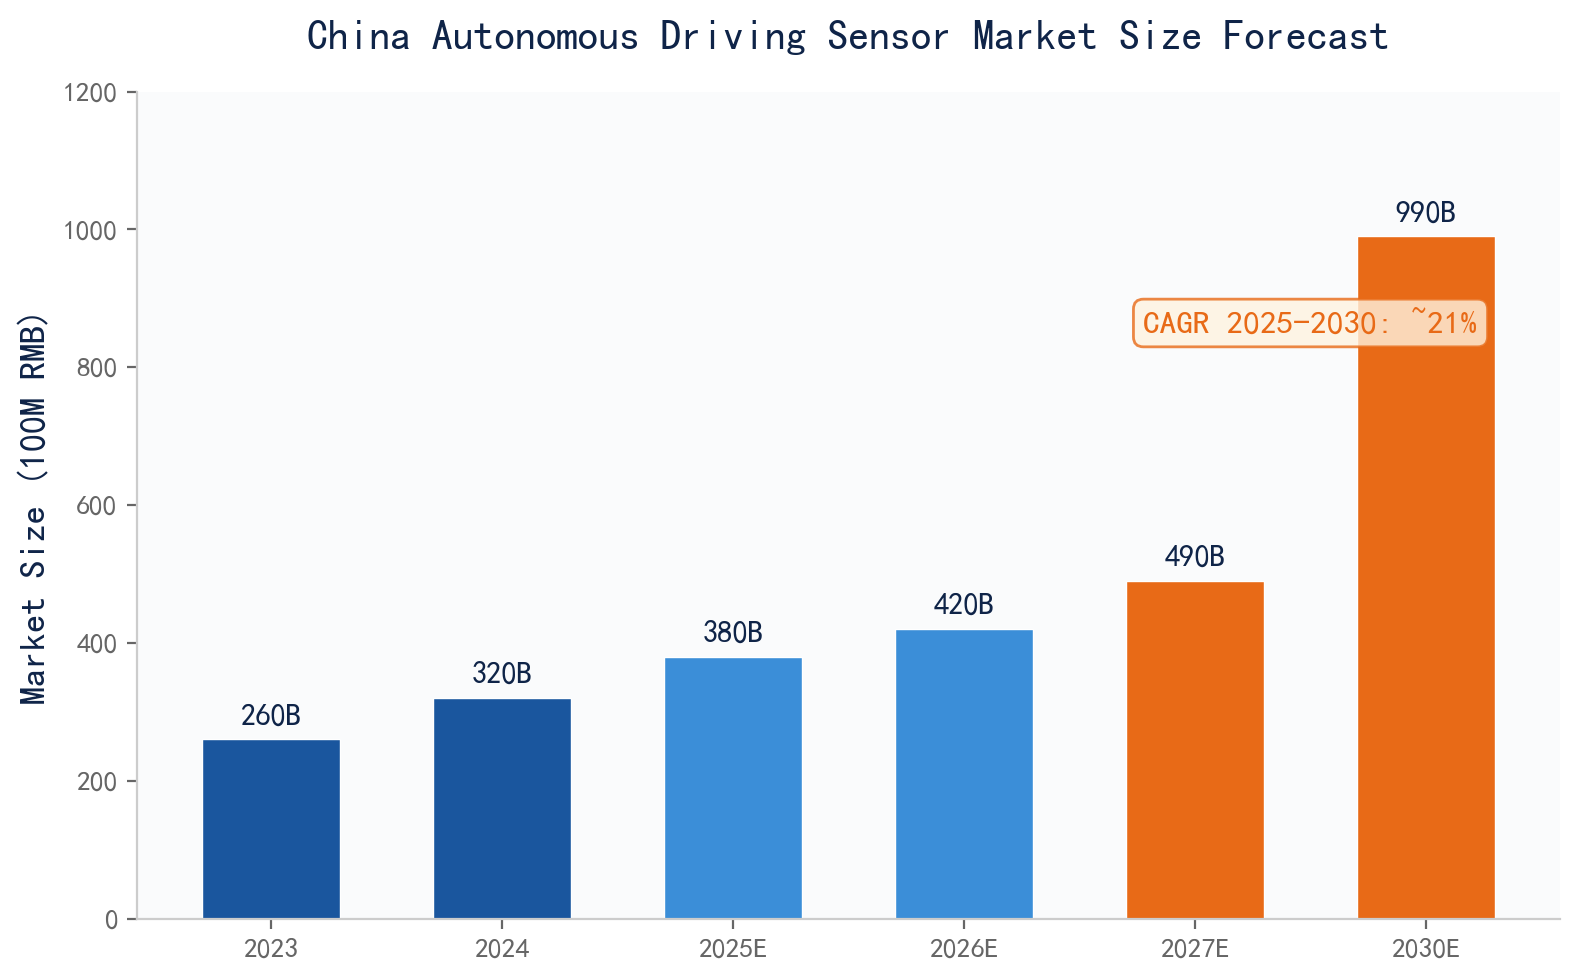
\includegraphics[width=0.88\textwidth]{figure/market_size.png}
\caption{中国自动驾驶传感器市场规模及预测（2023-2030）}
\label{fig:market_size}
\end{figure}

\keybox{2025-2030年中国自动驾驶传感器市场CAGR约21\%，激光雷达占比将从28\%跃升至45\%，成为市场份额最大的单一传感器品类。}

\section{核心传感器细分市场分析}

\subsection{激光雷达市场}

2024年全球激光雷达市场规模约512亿元，预计2027年突破千亿元。禾赛科技、速腾聚创在全球车载前装市场占据主导地位，国产激光雷达全球市占率约45\%-50\%。主激光雷达模组成本已从2020年的数万元降至2024年的3000-5000元，预计2027年将进一步下探至1500元以内。

\subsection{毫米波雷达市场}

2024年中国车载毫米波雷达前装搭载量超1800万颗（同比+27.6\%），市场规模约86亿元。4D成像毫米波雷达自2024年起进入大规模商用元年，77GHz CMOS雷达芯片已初步实现国产化替代（加特兰微电子Alps系列等）。

\subsection{车载摄像头市场}

车载摄像头是单车搭载数量最多的传感器（L2级5-8颗，L3/L4级12-15颗+）。2024年全球车载摄像头市场规模约170亿美元。韦尔股份（OmniVision）、格科微等在车载CIS领域已具备全球竞争力。

\section{典型企业及岗位分析}

\subsection{其域创新（XGRIDS）—— 3D激光雷达与空间数字化}

其域创新（XGRIDS, \url{https://xgrids.cn}）是一家专注于三维空间数字化技术的公司，以自研的固态激光雷达和多传感器融合算法为核心竞争力。其产品线覆盖高精度手持三维扫描仪、机载LiDAR系统及自动驾驶感知解决方案。该公司在激光雷达3D重建与多传感器融合领域有深厚的工程积累，其招聘岗位直接反映了产业界对传感器技术复合型人才的具体需求：

\textbf{（1）多传感器标定算法工程师}：负责激光雷达、摄像头、IMU、GNSS等多传感器之间的内参和外参标定算法研发。核心工作包括：基于PnP/手眼标定的LiDAR-Camera联合标定；多激光雷达之间的点云配准与SLAM轨迹优化。要求精通非线性优化理论（Ceres/G2O）、多视图几何及C++/Python编程。\par
\smallskip
{\footnotesize\color{gray}岗位链接：\url{https://pecivkvtit.jobs.feishu.cn/index/position/7486766416390113587/detail}\par}

\textbf{（2）感知融合算法工程师}：负责多模态感知数据的融合与目标检测算法开发。核心工作包括：基于BEV/Top-down视角的多传感器特征级融合；多目标跟踪（MOT）与轨迹预测算法；深度学习模型在嵌入式平台上的轻量化部署。要求熟悉PointPillars/CenterPoint等点云检测框架及PyTorch/TensorRT生态。\par
\smallskip
{\footnotesize\color{gray}岗位链接：\url{https://pecivkvtit.jobs.feishu.cn/index/position/7491253117397387529/detail}\par}

\textbf{（3）多传感器融合算法工程师（视觉雷达联合重建方向）}：聚焦于视觉与LiDAR的联合三维场景重建，包括NeRF/3D Gaussian Splatting等前沿方法，用于高精地图构建与数字孪生。该岗位代表了传感器感知与三维视觉交叉的最新前沿方向。\par
\smallskip
{\footnotesize\color{gray}岗位链接：\url{https://pecivkvtit.jobs.feishu.cn/index/position/7535787737665538350/detail}\par}

\subsection{禾赛科技与速腾聚创}

禾赛科技（Hesai Technology）和速腾聚创（RoboSense）是全球车载激光雷达出货量排名前两位的企业。禾赛AT128（128线混合固态激光雷达）2023年单年出货超40万台，创造全球纪录。速腾聚创的E1平台采用自研SPAD阵列与VCSEL发射方案，实现了低于500美元的系统成本。这些企业的人才需求涵盖光电芯片设计、ASIC电路设计、点云算法、嵌入式系统工程、自动驾驶系统集成等方向，为光电信息科学与工程、电子科学与技术、自动化、计算机科学等专业背景的毕业生提供了广阔的职业通道。

\clearpage

% ===================== 第2章 视觉摄像机 =====================
\chapter{视觉摄像机传感器}

\section{工作原理}

车载视觉摄像机是自动驾驶感知系统中最基础、最成熟的传感器。其核心是一块CMOS（互补金属氧化物半导体）图像传感器芯片，基于内光电效应（Internal Photoelectric Effect）实现光信号到电信号的转换。

\subsection{光电转换的物理基础}

当光子入射到半导体材料（通常为硅）表面时，若光子能量$E = h\nu$大于硅的禁带宽度$E_g \approx 1.12\ \text{eV}$，则价带中的电子被激发跃迁至导带，形成电子-空穴对。在PN结耗尽层中，内建电场将光生电子-空穴对分离，产生光电流$I_{ph}$。光电流与入射光功率$P_{opt}$的关系为：

\begin{equation}\label{eq:photocurrent}
I_{ph} = R \cdot P_{opt} = \frac{\eta q}{h\nu} \cdot P_{opt}
\end{equation}
式中，$R$为响应度（A/W），$\eta$为量子效率，$q$为电子电荷量。

\subsection{CMOS有源像素结构（4T-APS）}

现代车载CMOS图像传感器普遍采用4T-APS（4-Transistor Active Pixel Sensor）结构。每个像素包含四个晶体管：复位管（RST）、传输管（TX）、源跟随器（SF）和行选择管（RS），以及一个 pinned 光电二极管（PPD）。PPD的引入有效消除了传统PN结光电二极管的复位噪声（kTC噪声），使相关双采样（CDS）技术成为可能。

\section{核心元器件}

\subsection{相关双采样（CDS）降噪原理}

CMOS图像传感器的主要噪声源包括像素复位噪声（kTC噪声）、固定模式噪声（FPN）和暗电流散粒噪声。CDS技术通过对同一像素在复位电平（参考信号）与信号电平之间进行两次采样并做差，能够有效消除复位噪声和像素间的固定模式噪声：

\begin{equation}\label{eq:cds}
V_{out} = V_{signal} - V_{reset}
\end{equation}

这一差分操作是CMOS图像传感器信号链中最核心的噪声抑制电路设计。

\subsection{列级ADC架构}

为了将模拟像素信号转换为数字图像数据，CMOS图像传感器在每个像素列上集成一个列级ADC（Column-Parallel ADC）。主流架构包括：
\begin{itemize}
    \item \textbf{单斜ADC（Single-Slope ADC）}：结构简单，面积小，适用于高分辨率传感器，但转换速率受限于比较器时钟频率。
    \item \textbf{SAR ADC（逐次逼近型ADC）}：功耗效率高，适用于高帧率应用，已广泛用于最新一代车载CIS产品。
\end{itemize}

\section{车载摄像头的分类与应用}

\begin{table}[htbp]
\centering
\caption{车载摄像头分类与典型应用}
\label{tab:camera_types}
\begin{tabular}{cccl}
\toprule
\textbf{类型} & \textbf{视场角} & \textbf{分辨率} & \textbf{主要功能} \\
\midrule
前视单目 & 30\textdegree-60\textdegree & 2-8MP & FCW、LDW、TSR、ACC \\
前视双目/三目 & 30\textdegree-120\textdegree & 2-8MP & 立体视觉测距、AEB \\
环视（鱼眼） & 180\textdegree-190\textdegree & 1-3MP & 360\textdegree\ 全景泊车、BSD \\
DMS舱内摄像头 & 60\textdegree-90\textdegree & 1-2MP & 驾驶员疲劳监测、分心检测 \\
后视摄像头 & 130\textdegree-150\textdegree & 1-2MP & 倒车影像、RVC \\
\bottomrule
\end{tabular}
\end{table}

\section{车载摄像头的关键技术挑战}

\begin{enumerate}
    \item \textbf{高动态范围（HDR）}：车载场景需要同时处理夜间弱光（<1 lux）和日间强光（>100,000 lux），要求HDR达到120-140dB。主流技术方案包括多重曝光合成（SME-HDR）和分像素双转换增益（DCG-HDR）。
    \item \textbf{LED闪烁抑制（LFM）}：LED交通信号灯和车灯以PWM方式工作，若曝光时间不匹配，会导致图像中出现闪烁或黑块。车载CIS需要支持LFM模式，避免长曝光期间LED周期的盲区。
    \item \textbf{温度稳定性}：车载环境温度范围宽（-40\textdegree C至+105\textdegree C），暗电流随温度呈指数增长，需要片上温度补偿机制。
\end{enumerate}

\clearpage

% ===================== 第3章 毫米波雷达 =====================
\chapter{毫米波雷达传感器}

\section{工作原理}

车载毫米波雷达是自动驾驶感知系统中不可或缺的全天候传感器。其工作频段主要位于24GHz（窄带，短距）和76-81GHz（宽带，长距）两个频段。国际上，24GHz频段正逐步被替代，77GHz和79GHz已成为车载毫米波雷达的主流频段。

\subsection{FMCW信号模型}

主流车载毫米波雷达采用调频连续波（Frequency Modulated Continuous Wave, FMCW）体制。发射信号为线性调频信号（chirp）：

\begin{equation}\label{eq:fmcw_tx}
s_{TX}(t) = A_T \cos\left[2\pi\left(f_c t + \frac{B}{2T_c} t^2\right) + \phi_0\right], \quad 0 \leq t \leq T_c
\end{equation}
式中，$f_c$为起始频率（77GHz），$B$为调频带宽（通常为200MHz-4GHz），$T_c$为chirp周期。

发射信号经目标反射后，接收信号相对于发射信号存在时延$\tau = 2R/c$：

\begin{equation}\label{eq:fmcw_rx}
s_{RX}(t) = A_R \cos\left[2\pi\left(f_c (t - \tau) + \frac{B}{2T_c} (t - \tau)^2\right) + \phi_0\right]
\end{equation}

\subsection{混频与中频信号处理}

接收信号与发射信号的本振（LO）副本在混频器（Mixer）中相乘，经低通滤波后得到中频（IF）信号。其频率$f_{IF}$包含目标的距离信息，相位变化则包含速度信息：

\begin{equation}\label{eq:fmcw_if}
f_{IF} = \frac{2B \cdot R}{c \cdot T_c}
\end{equation}

由此可反演目标距离：
\begin{equation}\label{eq:fmcw_range}
R = \frac{c \cdot T_c \cdot f_{IF}}{2B}
\end{equation}

当目标具有径向相对速度$v_r$时，根据多普勒效应，回波载频偏移$f_d = 2v_r / \lambda$。通过发射多个chirp形成"快时间-慢时间"二维信号矩阵，经二维FFT（Range-Doppler FFT）即可同时提取目标的距离和速度信息。

\subsection{角度估计与4D成像雷达}

传统毫米波雷达通过多个接收天线组成的虚拟阵列，利用到达角（AoA）估计目标的方位角。对于包含$N_{TX}$个发射天线和$N_{RX}$个接收天线的MIMO阵列，可形成等效$N_{TX} \times N_{RX}$个虚拟接收通道。到达角$\theta$通过相邻天线间的相位差估计：

\begin{equation}\label{eq:aoa}
\theta = \arcsin\left(\frac{\lambda \cdot \Delta\phi}{2\pi \cdot d}\right)
\end{equation}

其中，$d$为天线间距，$\Delta\phi$为相邻通道间的相位差。传统的3D毫米波雷达仅能获得目标的距离-方位角-多普勒信息。而4D成像雷达通过增加俯仰向天线阵列（MIMO垂直维度），额外获得目标的高度信息，使雷达拥有"成像级"的点云输出能力，可有效识别静止障碍物、路沿和桥梁。

\section{核心元器件}

\subsection{77GHz MMIC收发芯片}

毫米波雷达的核心是单片微波集成电路（MMIC），集成了以下关键功能模块：

\begin{itemize}
    \item \textbf{频率合成器/锁相环（PLL）}：利用分数N分频锁相环产生高线性度的线性调频信号。chirp的线性度直接决定了雷达的距离分辨率$\Delta R = c/(2B)$。
    \item \textbf{功率放大器（PA）}：将微弱的chirp信号放大至足够功率后馈送至发射天线。
    \item \textbf{低噪声放大器（LNA）}：接收链路第一级，其噪声系数决定了雷达的整体灵敏度。
    \item \textbf{混频器（Mixer）与中频链路}：将毫米波信号下变频至基带/中频，然后经可编程增益放大器（PGA）和抗混叠低通滤波器后，由ADC进行数字化采样。
\end{itemize}

\subsection{CMOS工艺与国产替代}

近年来，77GHz CMOS毫米波雷达芯片取得了重大突破。传统的SiGe BiCMOS工艺虽然射频性能优异，但成本高且难以与数字基带集成。CMOS工艺（如28nm/45nm RF-CMOS）使MMIC与数字信号处理（DSP/MCU）的单芯片集成（SoC）成为可能，大幅降低了雷达模组的成本和小型化程度。

国产厂商加特兰微电子（Calterah）的77GHz/79GHz Alps系列CMOS毫米波雷达SoC已实现大规模量产供货。森思泰克、楚航科技等模组厂商也相继推出了基于国产芯片方案的4D成像雷达产品，推动车载毫米波雷达国产化率从2021年的不足10\%提升至2025年的约35\%。

\section{毫米波雷达的性能优势与局限}

\textbf{核心优势：}
\begin{itemize}
    \item 全天候工作能力：毫米波在雨、雾、雪、烟尘中的衰减远小于激光和可见光，是恶劣天气下最可靠的传感器。
    \item 速度测量直接且精准：通过多普勒效应直接获取目标的径向速度，无需帧间差分计算。
    \item 成本相对较低：单颗77GHz前雷达成本已降至200-400元区间。
\end{itemize}

\textbf{主要局限：}
\begin{itemize}
    \item 对静止物体的检测能力弱：难以区分静止车辆与金属护栏、路牌等（4D成像雷达正在改善此问题）。
    \item 角度分辨率有限：受天线孔径限制，方位角分辨率通常为1\textdegree-3\textdegree，远低于激光雷达（0.1\textdegree\ 级）。
    \item 对非金属目标（行人等）反射较弱：人体对毫米波的雷达截面积（RCS）远小于车辆。
\end{itemize}

\clearpage

% ===================== 第4章 超声波雷达 =====================
\chapter{超声波雷达传感器}

\section{工作原理}

超声波雷达（Ultrasonic Sensor）是汽车电子系统中应用最广泛的近距离传感器。其核心工作原理基于压电效应（Piezoelectric Effect）与脉冲回波法（Pulse-Echo Method）。

\subsection{压电换能器}

超声波传感器的核心换能元件为压电陶瓷片（如PZT-4/PZT-8系列锆钛酸铅陶瓷）。当在压电陶瓷两侧施加交变电压时，陶瓷片将产生与电压频率一致的机械振动，从而向空气中辐射超声波（逆压电效应）。当接收到的超声回波作用于陶瓷片上时，机械振动转换为电荷输出（正压电效应）。车载超声波传感器通常工作于40-58kHz频段，该频段的选择是探测距离、方向性和抗环境噪声之间的折中。

\subsection{渡越时间测距模型}

传感器发射一组超声波脉冲（通常为8-16个周期），脉冲经空气传播至障碍物后反射回来。设发射时刻为$t_0$，回波到达时刻为$t_1$，声速为$v_s$（空气中约340m/s），则障碍物距离为：

\begin{equation}\label{eq:ultrasonic_range}
R = \frac{1}{2} v_s \cdot (t_1 - t_0) = \frac{1}{2} v_s \cdot \Delta t
\end{equation}

\subsection{温度补偿}

声速$v_s$是温度的函数：
\begin{equation}\label{eq:sound_speed}
v_s(T) = 331.3 \times \sqrt{1 + \frac{T}{273.15}} \approx 331.3 + 0.606 \cdot T \ (\text{m/s})
\end{equation}
其中$T$为环境温度（\textdegree C）。车载超声波系统通常集成温度传感器以实时修正声速。

\section{测量电路：驱动与回波处理}

\subsection{发射驱动电路}

超声波发射需要数百伏的瞬时高压脉冲以驱动压电陶瓷产生足够的声压级。典型电路采用变压器升压拓扑或电荷泵（Charge Pump）升压方案：
\begin{itemize}
    \item \textbf{变压器方案}：利用中心抽头变压器的匝数比将MCU输出的低压脉冲（3.3V/5V）升压至100-300Vpp驱动换能器。
    \item \textbf{集成驱动方案}：现代自动泊车系统（APA）中的超声波传感器采用ASIC集成驱动芯片，如Elmos E524系列，内部集成了升压DCDC、脉冲发生器和回波接收放大链路。
\end{itemize}

\subsection{回波接收与阈值检测}

接收链路包括以下关键模块：
\begin{enumerate}
    \item \textbf{低噪声前置放大器（LNA）}：将压电换能器输出的微伏至毫伏级回波信号进行初级放大。
    \item \textbf{带通滤波器（BPF）}：中心频率40-58kHz，带宽2-5kHz，抑制发动机噪声、风噪等带外干扰。
    \item \textbf{可变增益放大器（VGA）}：补偿信号随距离增加而指数衰减的物理特性，实现接收灵敏度的时间-增益控制（TGC）。
    \item \textbf{阈值比较器/ADC}：将处理后的模拟信号与设定阈值比较，产生数字脉冲触发时间戳记录。
\end{enumerate}

\section{应用场景与性能边界}

超声波雷达广泛应用于：
\begin{itemize}
    \item \textbf{UPA（泊车辅助）}：探测距离0.3-2.5m，传感器安装于前后保险杠。
    \item \textbf{APA（自动泊车辅助）}：探测距离0.3-5m，需要更多传感器（8-12颗）和侧向安装。
    \item \textbf{BSD（盲区检测辅助）}：使用长距超声波传感器（探测距离可达5-7m）。
\end{itemize}

其性能边界包括：探测距离短（$\leq$7m）、方向性差（波束角约60\textdegree-120\textdegree）、受风噪/雨滴撞击干扰大、声速因温度变化引入距离误差等。

\clearpage

% ===================== 第5章 激光雷达 =====================
\chapter{激光雷达（LiDAR）传感器}

激光雷达（Light Detection and Ranging, LiDAR）是L3+自动驾驶感知系统的核心传感器，也是当前技术迭代最快、资本密集度最高的传感器赛道。本章从物理原理到测量电路进行系统性深入分析。

\section{工作原理}

\subsection{内光电效应与单光子探测}

激光雷达接收端的物理基础是内光电效应。当波长为$\lambda$的激光光子入射到半导体探测器表面时，若光子能量$E = hc/\lambda$大于半导体材料的禁带宽度$E_g$，价带电子被激发至导带，形成电子-空穴对。在外部反向偏置高压的作用下，这些光生载流子在耗尽层强电场中被加速漂移，产生可测量的光电流。

对于1550nm波长的激光，光子能量$E \approx 0.80\ \text{eV}$，InGaAs材料的$E_g \approx 0.75\ \text{eV}$，可以满足内光电效应的能量条件。而对于905nm波长，$E \approx 1.37\ \text{eV}$，硅基材料（$E_g \approx 1.12\ \text{eV}$）完全适用。

\subsection{飞行时间法（ToF）测距模型}

ToF（Time of Flight）是当前量产固态激光雷达最成熟的测距体制。发射端发出一束极窄的脉冲激光（脉宽$\tau_p$通常为1-10ns），目标反射的回波经自由空间传播后到达接收端。距离$R$由激光往返时间$\Delta t$计算：

\begin{equation}\label{eq:lidar_tof}
R = \frac{1}{2} c \cdot \Delta t
\end{equation}

其中$c = 3 \times 10^8\ \text{m/s}$为光速。要达到1cm的测距精度，$\Delta t$的测量精度需达到约66.7ps（皮秒）——这对时间测量电路提出了极高的要求。

\subsection{调频连续波（FMCW）激光雷达}

FMCW体制的激光雷达与FMCW毫米波雷达共享相同的数学模型基础，但在光学域实现。发射激光的频率随时间线性变化（通过调制激光器的注入电流或使用外部调制器），回波与本振光在光学混频器中产生拍频（beat note）。目标距离和速度分别由拍频的中频分量和多普勒频移决定：

\begin{equation}\label{eq:lidar_fmcw_r}
f_{IF} = \frac{2B \cdot R}{c \cdot T_m},\quad f_d = \frac{2v_r}{\lambda}
\end{equation}

FMCW激光雷达的核心优势在于：
\begin{enumerate}
    \item \textbf{抗干扰}：仅对与本振光频率匹配的信号产生响应，天然免疫其他激光雷达的脉冲串扰和阳光干扰。
    \item \textbf{同时测距测速}：无需帧间差分即可获取目标的径向速度。
    \item \textbf{灵敏度高}：相干接收的散粒噪声极限远低于直接探测。
\end{enumerate}

其技术瓶颈在于需要窄线宽（kHz级）、频率可线性调谐的激光器，以及高带宽的光学混频和平衡探测器，系统复杂度和成本显著高于ToF方案。

\section{核心元器件}

\subsection{发射端：从EEL到VCSEL到多结VCSEL}

\begin{itemize}
    \item \textbf{边发射激光器（EEL）}：传统方案，光束从芯片侧面出射，难以形成二维阵列，适合旋转式/转镜式机械扫描雷达。
    \item \textbf{垂直腔面发射激光器（VCSEL）}：光束垂直于芯片表面出射，可实现大规模二维阵列的晶圆级制造和测试，是固态Flash激光雷达和可寻址VCSEL阵列的核心光源。905nm VCSEL（GaAs基）已实现多结（Multi-Junction）堆叠，在保持人眼安全等级的前提下将峰值功率密度提升了3-5倍。
\end{itemize}

波长选择存在905nm与1550nm两大技术路线的竞争。1550nm（InP基）的光源远离人眼视网膜吸收带，允许发射更高的激光功率，因此探测距离更远。但其探测器（InGaAs APD/SPAD）成本高于硅基方案。905nm方案凭借硅基探测器的成本优势在现阶段的中短距ADAS市场占据主导。

\subsection{接收端：从PIN到APD到SPAD/SiPM}

探测器从普通PIN光电二极管到雪崩光电二极管（APD），再到单光子雪崩二极管（SPAD），其灵敏度逐步提高了数个数量级：

\begin{itemize}
    \item \textbf{PIN光电二极管}：无内部增益，响应度为0.4-0.8 A/W（Si@905nm），仅适用于近距离强回波场景。
    \item \textbf{APD（雪崩光电二极管）}：工作于线性模式，施加的反向偏压低于击穿电压。光生载流子在耗尽层高电场中被加速，通过碰撞电离产生链式倍增（雪崩效应），增益$M$通常为50-200倍。
    \item \textbf{SPAD（单光子雪崩二极管）}：工作于Geiger模式，偏压高于击穿电压。此时APD进入非线性的雪崩击穿状态——单个入射光子即可触发出宏观的雪崩电流。SPAD的探测灵敏度达到量子极限。
    \item \textbf{SiPM（硅光电倍增管）}：由成千上万个独立SPAD微单元并联组成。每个微单元串联一淬灭电阻，雪崩发生后自动复位。SiPM的宏观输出电流正比于同时触发雪崩的微单元数量，从而在保留SPAD单光子灵敏度的同时获得了光子数分辨能力（动态范围）。
\end{itemize}

\subsection{固态扫描器件：MEMS与OPA}

实现三维空间覆盖需要光束扫描机制。固态方案主要有两种技术路线：

\begin{itemize}
    \item \textbf{MEMS微振镜}：利用MEMS工艺制造的微米级硅基反射镜，在电磁或静电力驱动下发生二维偏转，改变光路方向。MEMS振镜已成功应用于禾赛AT128（一维转镜+MEMS二维扫描）等量产产品。其反射镜的谐振频率通常为1-2kHz（快轴）和几十Hz（慢轴），可实现类似利萨如（Lissajous）或光栅扫描的扫描图案。
    \item \textbf{光学相控阵（OPA）}：利用集成光波导阵列中的热光或电光效应，通过改变各波导通道中光的相对相位，在远场利用多光束干涉原理实现光斑的无惯性扫描（Beam Steering）。OPA是理想的"纯固态"方案，没有任何可动部件。但当前OPA受限于波导损耗、串扰和光栅瓣（Grating Lobe）等物理问题，水平和垂直视场角分别约为40\textdegree\ 和20\textdegree，尚不能满足车载全视场扫图的需求。
\end{itemize}

\section{高精度微弱信号测量电路}

\subsection{跨阻放大器（TIA）——光电信号的前端调理}

光电探测器（APD/SPAD/SiPM）输出的信号是极其微弱的电流脉冲（典型峰值在微安至毫安量级，脉宽在纳秒级）。跨阻放大器（Transimpedance Amplifier, TIA）是连接探测器与后续数字电路之间的关键桥梁，其基本功能是将微弱电流信号转换为可被ADC或TDC处理的电压信号。

理想TIA的输出为：
\begin{equation}\label{eq:tia_basic}
V_{out} = -I_{in} \cdot R_f
\end{equation}
其中$R_f$为反馈电阻。然而，在实际高频电路中，光电二极管的结电容$C_d$与反馈电阻$R_f$形成RC低通极点，限制了TIA的带宽。要保证纳秒级脉冲的保真度，TIA的闭环带宽$f_{-3dB}$需满足：
\begin{equation}\label{eq:tia_bw}
f_{-3dB} \geq \frac{0.35}{t_r} \ (\text{其中}t_r\text{为脉冲上升时间})
\end{equation}

对于$t_r = 1$ns的脉冲，TIA带宽需达到350MHz以上。为实现高增益与高带宽的兼顾，需要在$R_f$两端并联补偿电容$C_f$以引入零点补偿。TIA的闭环传递函数为：
\begin{equation}\label{eq:tia_transfer}
H(s) = \frac{V_{out}(s)}{I_{in}(s)} = -\frac{R_f}{1 + s \cdot R_f C_f}
\end{equation}

通过选择$C_f$使得$R_f C_f$匹配输入端的RC时间常数，可获得最大平坦带宽（Butterworth响应）。此时最佳补偿条件为：
\begin{equation}\label{eq:tia_comp}
C_f = \sqrt{\frac{C_d}{2\pi \cdot GBW \cdot R_f}}
\end{equation}
其中$GBW$为运算放大器的增益带宽积。

\textbf{TIA噪声分析模型。}TIA的等效输入噪声电流谱密度$\overline{i_{n,in}^2}$主要由三部分构成：
\begin{equation}\label{eq:tia_noise}
\overline{i_{n,in}^2} = \underbrace{\frac{4kT}{R_f}}_{\text{反馈电阻热噪声}} + \underbrace{\overline{e_n^2} \cdot \left(\frac{1}{R_f^2} + (2\pi f)^2 (C_d + C_f)^2\right)}_{\text{运放输入电压噪声的增益放大}} + \underbrace{\overline{i_n^2}}_{\text{运放输入电流噪声}}
\end{equation}
式中$k = 1.38 \times 10^{-23}\ \text{J/K}$为玻尔兹曼常数，$T$为绝对温度，$\overline{e_n^2}$和$\overline{i_n^2}$分别为运放的输入电压和电流噪声谱密度。式(\ref{eq:tia_noise})揭示了TIA设计的核心矛盾：增大$R_f$可降低反馈电阻的热噪声贡献（$4kT/R_f$），但同时增加了输入电压噪声通过寄生电容的耦合放大效应（因带宽减小导致高频噪声积分窗口变化）。在先进CMOS工艺中，通过采用共源共栅（Cascode）输入级和噪声抵消技术，可将等效输入噪声压低至$1.5-3.0\ \text{pA}/\sqrt{\text{Hz}}$量级。

\textbf{TIA的输入-输出信噪比链路预算。}以905nm激光雷达为典型场景：设发射峰值功率$P_{peak} = 100\ \text{W}$，目标距离$R = 100\ \text{m}$，目标反射率$\rho = 0.1$（朗伯反射体），接收光学孔径$D = 20\ \text{mm}$。根据激光雷达方程：
\begin{equation}\label{eq:lidar_eq}
P_{rx} = P_{peak} \cdot \rho \cdot \frac{A_{rx}}{R^2} \cdot \eta_{opt} \cdot \eta_{atm} \cdot \cos\theta
\end{equation}
其中$A_{rx} = \pi D^2/4$为接收面积，$\eta_{opt}$为光学系统透过率（典型0.7-0.9），$\eta_{atm}$为大气透过率（905nm处约0.6-0.8/km），$\theta$为目标表面法线与入射光夹角。代入典型参数计算得$P_{rx} \approx 1.57 \times 10^{-7}\ \text{W}$（约157nW）。若SPAD的探测效率（PDE）为10\%，则到达探测器的光子数率为$n_{ph} = P_{rx} \cdot PDE / (hc/\lambda) \approx 7.1 \times 10^{10}\ \text{photons/s}$。TIA需在此动态范围内保持线性放大，同时保证输出信噪比$SNR \geq 10$以满足后续TDC的触发阈值判别需求。

\begin{table}[htbp]
\centering
\caption{先进TIA集成芯片性能对比}
\label{tab:tia_comparison}
\begin{tabular}{ccccc}
\toprule
\textbf{文献} & \textbf{工艺节点} & \textbf{带宽} & \textbf{输入噪声} & \textbf{功耗/通道} \\
\midrule
文献[方吉鑫等,2026] & 180nm CMOS & 900MHz & 2.5pA/$\sqrt{\text{Hz}}$ & 1.5mW \\
文献[林远启等,2021] & SiGe BiCMOS & 200MHz & 3.2pA/$\sqrt{\text{Hz}}$ & 3.5mW \\
某国际厂商前端芯片 & 65nm CMOS & 750MHz & 1.8pA/$\sqrt{\text{Hz}}$ & 1.2mW \\
\bottomrule
\end{tabular}
\end{table}

\subsection{时间数字转换器（TDC）——皮秒级时间间隔测量}

TDC是ToF激光雷达测距精度的决定性电路。对于1cm的距离分辨率需求，时间测量精度必须达到约67ps。传统基于时钟计数器的方法受限于系统时钟频率（几百MHz量级，对应几纳秒分辨率），无法满足皮秒级精度要求。

\textbf{抽头延迟线型TDC}利用基本门电路（缓冲器/反相器）的传播延迟作为精细时间刻度。Start信号在一串串联缓冲器（延迟线）中传播，每个缓冲器产生固定的小延迟$\tau_{LSB}$（在先进CMOS工艺中可达10-20ps）。当Stop信号（回波到达）到来时，触发一组D触发器锁存延迟线上每个抽头的当前逻辑状态。设被记录的"1"的个数为$N$，则精细时间间隔为：

\begin{equation}\label{eq:tdc_fine}
\Delta t_{fine} = N \cdot \tau_{LSB}
\end{equation}

\textbf{Vernier型TDC}则采用两条具有微小延迟差的延迟线（如$\tau_1 = 50$ps，$\tau_2 = 48$ps），利用游标卡尺的"对齐"原理将分辨率进一步提高至$\tau_1 - \tau_2 = 2$ps的量级。

\textbf{TDC计时精度与测距误差分析。}TDC的单次测量精度受多个误差源限制。总计时抖动$\sigma_{TDC}$可建模为：
\begin{equation}\label{eq:tdc_jitter}
\sigma_{TDC} = \sqrt{\sigma_{q}^2 + \sigma_{DNL}^2 + \sigma_{PVT}^2 + \sigma_{walk}^2}
\end{equation}
其中$\sigma_{q} = \tau_{LSB}/\sqrt{12}$为量化误差（均匀分布假设），$\sigma_{DNL}$为延迟线微分非线性（DNL）引入的累积偏差，$\sigma_{PVT}$为工艺-电压-温度（PVT）波动引起的延迟漂移，$\sigma_{walk}$为由回波脉冲幅度变化导致的定时游走（Time Walk）误差——幅值较小的远距回波越过阈值比较器的时间晚于幅值较大的近距回波，即使两者的真实到达时间相同。

由TDC计时抖动$\sigma_{TDC}$通过ToF方程传播至距离误差：
\begin{equation}\label{eq:tdc_range_err}
\sigma_R = \frac{c}{2} \cdot \sigma_{TDC}
\end{equation}
以$\sigma_{TDC} = 30$ps为例，$\sigma_R \approx 4.5$mm。但考虑多次测量的统计平均效应，若采用多脉冲累加（如发射$N_p = 100$个脉冲并取ToF中值/均值），则测距精度可提升为$\sigma_R/\sqrt{N_p}$（白噪声假设下），即约0.45mm@100脉冲。实际系统中常采用基于直方图的统计算法（如时间相关单光子计数TCSPC），通过构建光子到达时间的统计直方图，以峰值检测或加权质心法提取高置信度的ToF估计值，在强背景光下仍可实现厘米级甚至毫米级的测距精度。

\subsection{SPAD光子探测的统计模型}

SPAD工作于Geiger模式，其对入射光子的响应具有概率统计特性。单个SPAD微单元在一次探测周期内发生雪崩的概率$P_{det}$服从非齐次泊松过程：
\begin{equation}\label{eq:spad_prob}
P_{det} = 1 - \exp\left(-\int_{0}^{T_g} [\eta_{PDE} \cdot \Phi_{ph}(t) + DCR] \cdot dt\right)
\end{equation}
式中$\eta_{PDE}$为光子探测效率（Photon Detection Efficiency，为量子效率$\eta_{QE}$与几何填充因子$FF$及雪崩触发概率$P_{av}$的乘积：$\eta_{PDE} = \eta_{QE} \cdot FF \cdot P_{av}$），$\Phi_{ph}(t)$为入射光子通量，$DCR$为暗计数率（单位：cps），$T_g$为门控时间窗口。

SiPM由$N_{micro}$个独立SPAD微单元并联组成，其宏观输出电流$I_{SiPM}$满足：
\begin{equation}\label{eq:sipm_current}
I_{SiPM} = \frac{N_{fired}}{N_{micro}} \cdot G_{SPAD} \cdot q
\end{equation}
其中$N_{fired}$为同时触发雪崩的微单元数，$G_{SPAD}$为单个SPAD的雪崩增益（典型$10^5-10^6$），$q$为电子电荷量。当$N_{fired} \ll N_{micro}$时（线性区），$I_{SiPM} \propto \Phi_{ph}$；当$N_{fired}$接近$N_{micro}$时，SiPM进入饱和区，输出-输入关系偏离线性。这一非线性效应需在系统标定中予以补偿。

\subsection{淬灭与复位电路（Quenching Circuit）}

SPAD在触发雪崩后需要主动淬灭和复位以准备下一次探测。淬灭电路分为：
\begin{itemize}
    \item \textbf{无源淬灭（Passive Quenching）}：串联一个大电阻或一个MOSFET电流源，雪崩电流在电阻上的压降使偏压降至击穿电压以下，自然淬灭。结构简单，但恢复时间（Dead Time）较长（数十ns到数百ns）。
    \item \textbf{主动淬灭（Active Quenching）}：通过高速反馈电路检测雪崩事件的发生，主动将偏压拉低，在雪崩结束后再主动恢复到工作偏压。恢复时间可压缩至几纳秒，适合高光子通量场景。
\end{itemize}

\section{暗电流与噪声分析}

暗电流（Dark Current）是限制弱光探测器性能的核心物理瓶颈。即使在完全无光的条件下，反向偏置的PN结中仍存在因热激发（Shockley-Read-Hall, SRH产生-复合过程）和带间隧穿而产生的微弱电流。暗电流$I_{dark}$的主要来源为：

\begin{equation}\label{eq:dark_current}
I_{dark} \propto n_i \propto T^{3/2} \exp\left(-\frac{E_g}{2kT}\right)
\end{equation}

暗电流对温度极为敏感——温度每升高约8-10\textdegree C，暗电流约翻一番。在车载高温环境（+85\textdegree C）下，暗电流可能比室温条件下高2-3个数量级。这导致SPAD的暗计数率（Dark Count Rate, DCR）急剧上升，产生大量虚假事件（噪声点云），严重恶化测距的置信度。

噪声抑制策略包括：芯片制造环节减少缺陷和杂质陷阱态；系统层面通过TEC热电制冷器将探测器温度稳定在25\textdegree C附近；算法层面通过时间符合滤波（Coincidence Filtering）剔除孤立暗计数触发。

\section{固态激光雷达全链路信号流图}

为直观展示固态激光雷达从光子发射到数字点云输出的完整物理链路，图\ref{fig:lidar_chain}以TikZ矢量图呈现了核心信号链：VCSEL阵列发射脉冲激光$\rightarrow$目标反射回波光子$\rightarrow$SPAD/SiPM单光子探测$\rightarrow$TIA跨阻放大（I$\rightarrow$V转换）$\rightarrow$TDC皮秒计时$\rightarrow$数字信号处理器生成3D点云。

\begin{figure}[htbp]
\centering
\begin{tikzpicture}[node distance=1.8cm, auto]
% VCSEL
\node[block_o] (vcsel) {VCSEL阵列\\905/1550nm\\脉冲激光源};
% Target
\node[block_gray, right=of vcsel] (target) {目标物体\\漫反射\\$\sigma$ RCS};
% SPAD
\node[block, right=of target] (spad) {SPAD/SiPM\\单光子探测器\\Geiger模式};
% TIA
\node[block, below=of spad, xshift=-1.5cm] (tia) {TIA跨阻放大器\\I$\rightarrow$V转换\\BW$\ge$350MHz};
% TDC
\node[block, right=of tia, xshift=1.5cm] (tdc) {TDC时间数字\\转换器 10-20ps\\皮秒级计时};
% DSP
\node[block_o, right=of tdc] (dsp) {数字信号处理器\\直方图/TCSPC\\3D点云输出};

% emission path
\draw[arr_o] (vcsel) -- (target) node[midway, lbl, above] {发射脉冲$\tau_p$=1-10ns};
% reflection path
\draw[arr_g] (target.south) -- ++(0,-1.5) -| (spad) node[pos=0.25, lbl, below] {回波光子};
% SPAD to TIA
\draw[arr] (spad.south) -- ++(0,-0.6) -| (tia) node[pos=0.5, lbl, left] {$\mu$A脉冲电流};
% TIA to TDC
\draw[arr] (tia) -- (tdc) node[midway, lbl, above] {mV级电压脉冲};
% TDC to DSP
\draw[arr_o] (tdc) -- (dsp) node[midway, lbl, above] {精确$\Delta$t (ps)};

% Annotation
\node[note, below=of tia, yshift=0.8cm] {SIP系统级封装};
\draw[arr_g, dashed] (spad.south west) -- ++(-0.4,-0.8) -| (tia.west);

\end{tikzpicture}
\caption{固态激光雷达全链路信号流：从光子发射到数字点云}
\label{fig:lidar_chain}
\end{figure}

\section{SIP系统级封装与信号完整性}

为了抑制PCB长走线引入的寄生电感和寄生电容对微弱高速信号的衰减，现代激光雷达接收系统广泛采用系统级封装（System in Package, SIP）技术，将探测器芯片与TIA芯片在物理空间上进行微米级的超短互连，封装于同一管壳内。SIP不仅消除了中间连接线上的寄生参数，而且减少了电磁干扰（EMI）接收面积。部分先进方案（如禾赛AT128的接收模块）将APD阵列、TIA阵列和初级ADC以3D堆叠（3D-Stacking）方式集成，采用TSV（硅通孔）实现垂直互连，极大提升了接收链路的信号完整性。

\clearpage

% ===================== 第6章 惯性传感器 =====================
\chapter{惯性测量单元（IMU）传感器}

\section{工作原理}

惯性测量单元（Inertial Measurement Unit, IMU）通过感知载体的加速度和角速度来推算载体的运动状态，是自动驾驶定位系统中的关键传感器。现代车载IMU几乎全部基于微机电系统（MEMS）技术制造。

\subsection{MEMS加速度计}

MEMS加速度计的基本原理是将加速度引起的惯性力转换为电容或压阻变化。以最主流的电容式MEMS加速度计为例，其核心结构是一个通过弹性悬臂梁支撑的硅基质量块（Proof Mass），质量块两侧设有固定梳齿电极。当载体沿敏感轴方向产生加速度$a$时，惯性力$F = m \cdot a$使质量块相对于固定电极产生位移$\Delta x$，引起差分电容$C_1$与$C_2$的变化：

\begin{equation}\label{eq:accel_cap}
\Delta C = C_1 - C_2 \propto \Delta x \propto a
\end{equation}

电容变化通过片上开关电容（Switched-Capacitor）读出电路转换为电压信号，经ADC后输出数字加速度值。

\subsection{MEMS陀螺仪}

MEMS振动陀螺仪利用科里奥利力（Coriolis Force）效应测量角速度。其结构包含一个在驱动方向上以恒定频率$\omega_d$振动的质量块。当载体绕垂直于驱动-检测平面的轴以角速度$\Omega$旋转时，质量块在检测方向上受到科里奥利力作用：

\begin{equation}\label{eq:coriolis}
F_c = -2m \cdot (\vec{\Omega} \times \vec{v})
\end{equation}

其中$m$为质量块质量，$\vec{v}$为质量块在驱动方向上的瞬时速度。科里奥利力使质量块在检测方向上产生与角速度$\Omega$成正比的位移，由电容检测电路读出。

\section{IMU的信号处理与误差模型}

\subsection{捷联惯导解算}

IMU以高频率（100-1000Hz）输出三轴加速度$(a_x, a_y, a_z)$和三轴角速度$(\omega_x, \omega_y, \omega_z)$。通过捷联惯导算法（Strapdown Inertial Navigation），计算机对角速度积分得到载体的姿态四元数/欧拉角，将加速度从载体坐标系旋转至导航坐标系，再经重力和科里奥利力补偿后进行二重积分，得到位置和速度估计。

\subsection{误差模型与零偏不稳定性}

MEMS-IMU的误差源主要包括：
\begin{itemize}
    \item \textbf{零偏（Bias）}：在无输入运动时传感器输出的非零均值，表现为陀螺仪零偏不稳定性（Bias Instability, 单位: $^\circ$/hr）和加速度计零偏。
    \item \textbf{比例因子误差（Scale Factor Error）}：传感器输出的斜率非线性。
    \item \textbf{交叉轴灵敏度（Cross-Axis Sensitivity）}：各敏感轴之间的耦合。
    \item \textbf{角度随机游走（Angle Random Walk, ARW）}：由热机械噪声引起的白噪声积分，单位为$^\circ/\sqrt{\text{hr}}$。
\end{itemize}

\textbf{Allan方差分析与噪声辨识。}MEMS-IMU各类误差源具有不同的时域相关特性，可通过Allan方差法在频域/时域进行有效分离和辨识。对于采样周期为$\tau_0$的$N$点陀螺仪/加速度计静态数据，将数据分为长度为$m$的$K$个簇（$m < N/2$），每个簇的平均值为$\bar{\Omega}_k(m)$。Allan方差定义为相邻簇均值之差的统计期望的一半：
\begin{equation}\label{eq:allan_var}
\sigma^2_A(\tau) = \frac{1}{2}\left\langle \left(\bar{\Omega}_{k+1}(m) - \bar{\Omega}_k(m)\right)^2 \right\rangle
\end{equation}
其中$\tau = m \cdot \tau_0$为积分时间。对Allan标准差$\sigma_A(\tau)$绘制双对数曲线（Allan Deviation Plot），不同斜率区域对应不同的噪声机制：
\begin{itemize}
    \item $\sigma_A(\tau) \propto \tau^{-1/2}$（斜率-1/2）：角度/速度白噪声（ARW/VRW）
    \item $\sigma_A(\tau) \propto \tau^{0}$（斜率0）：零偏不稳定性（Bias Instability，$1/f$闪烁噪声）
    \item $\sigma_A(\tau) \propto \tau^{+1/2}$（斜率+1/2）：角速率/加速度随机游走（RRW/RW）
    \item $\sigma_A(\tau) \propto \tau^{+1}$（斜率+1）：量化噪声（Quantization Noise）
    \item $\sigma_A(\tau)$在长积分时间处的极小值即为零偏不稳定性的定量指标（如$0.5^\circ/\text{hr}$、$2^\circ/\text{hr}$等）
\end{itemize}
Allan方差分析为MEMS-IMU选型和传感器融合算法中噪声参数的设置（如扩展卡尔曼滤波的$Q$矩阵）提供了关键的先验统计信息。典型车载战术级MEMS-IMU的零偏不稳定性在$0.5-5^\circ/\text{hr}$（陀螺仪）和$5-50\ \mu\text{g}$（加速度计）范围内。

\section{IMU与其他传感器的互补定位}

纯IMU的积分漂移在几十秒内就会使位置估计完全发散。因此，IMU在自动驾驶中从不单独使用，而是通过传感器融合与GPS/GNSS、视觉里程计（Visual Odometry, VO）和激光雷达里程计（LiDAR Odometry, LO）形成互补：
\begin{itemize}
    \item \textbf{GPS/IMU组合导航}：当GPS信号良好时（开阔道路），GPS提供绝对位置校正以抑制IMU漂移；当GPS信号中断时（隧道、城市峡谷），IMU提供短时高精度的航迹推算（Dead Reckoning）。
    \item \textbf{视觉-惯性里程计（VIO）}：利用连续图像帧间的特征匹配联合IMU预积分进行紧耦合位姿估计，提供高频位姿输出。
    \item \textbf{激光雷达-惯性里程计（LIO）}：利用点云配准与IMU预积分联合优化，如LIO-SAM框架，是当前高精地图构建和自动驾驶定位的主流方案。
\end{itemize}

\clearpage

% ===================== 第7章 多传感器融合 =====================
\chapter{多传感器融合与深度学习应用}

\section{多传感器融合的必要性}

如表\ref{tab:sensor_comp}所示，每一类传感器在工作原理、感知能力和失效模式上各有优劣，不存在单一种类的"全能"传感器。多传感器融合的根本目标是通过对异质传感器数据的时空对准与信息互补，实现任何单一传感器均无法达成的感知鲁棒性和准确性。

\begin{table}[htbp]
\centering
\caption{五大车载传感器综合性能对比}
\label{tab:sensor_comp}
\resizebox{\textwidth}{!}{%
\begin{tabular}{ccccccc}
\toprule
\textbf{性能维度} & \textbf{摄像头} & \textbf{毫米波雷达} & \textbf{超声波雷达} & \textbf{激光雷达} & \textbf{IMU} \\
\midrule
测距能力 & 中（双目） & 优 & 近距 & 最优（cm级） & 无 \\
速度测量 & 间接 & 直接（多普勒） & 无 & 直接（FMCW） & 间接（积分） \\
角度分辨率 & 优 & 中（1-2\textdegree） & 差 & 优（<0.1\textdegree） & N/A \\
纹理/颜色 & 最优 & 无 & 无 & 无（强度） & 无 \\
夜间/暗光 & 差 & 优 & 优 & 优（主动光源） & 优 \\
雨雾雪天 & 差 & 优 & 中 & 中-差 & 优 \\
成本（单颗） & \$10--50 & \$30--80 & \$5--15 & \$200--1000 & \$10--50 \\
\bottomrule
\end{tabular}%
}
\end{table}

\begin{figure}[htbp]
\centering
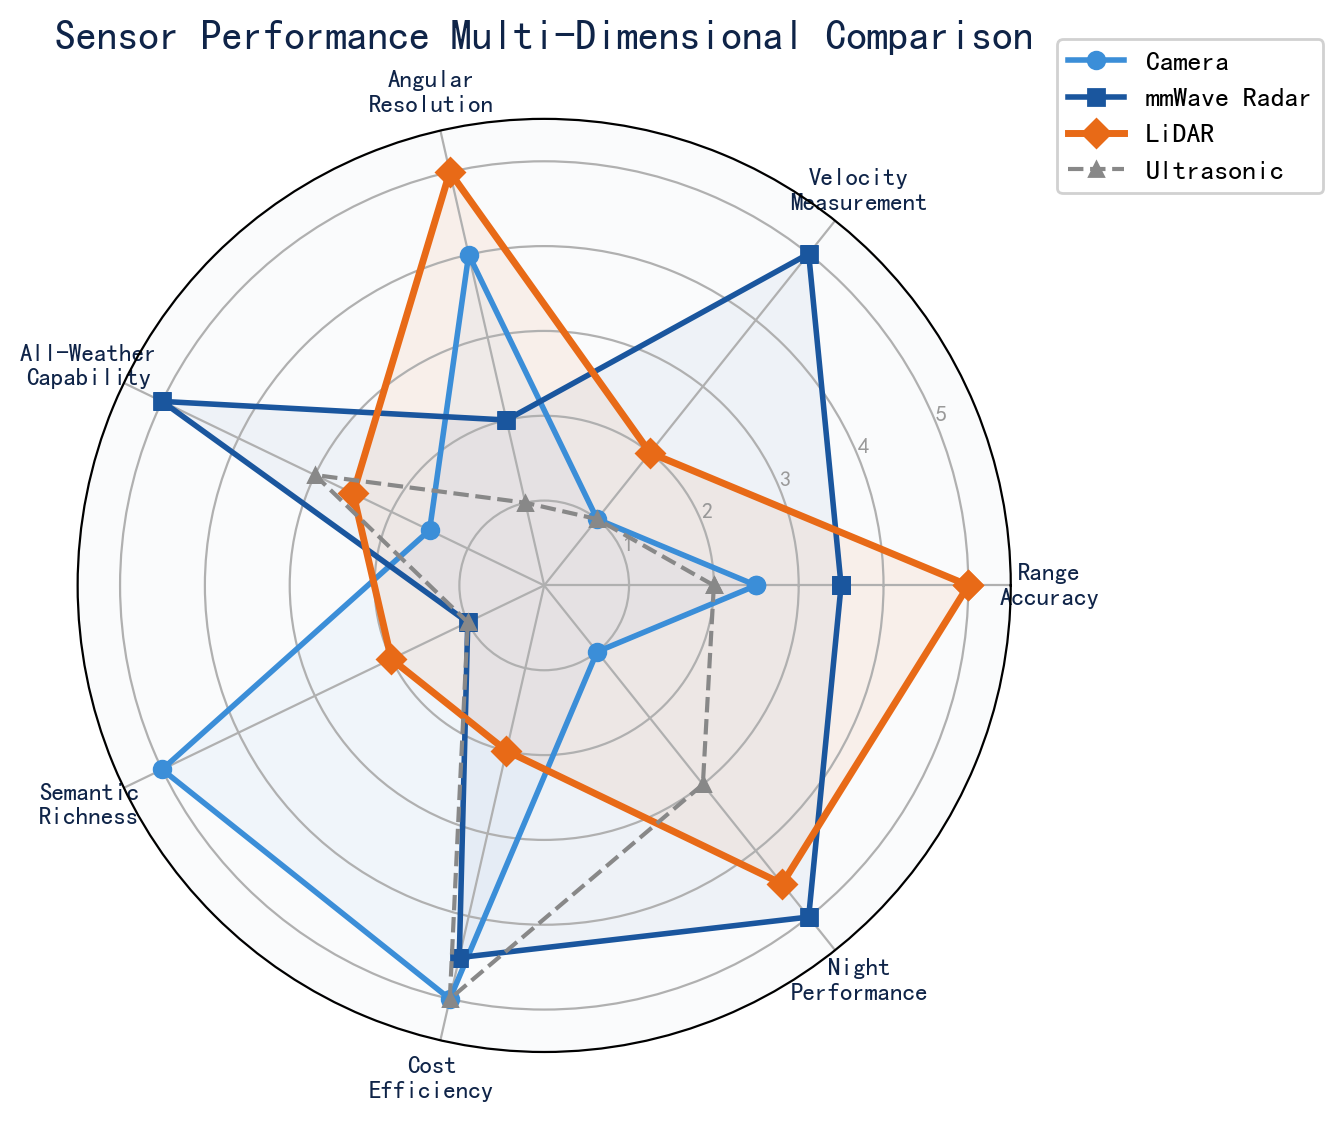
\includegraphics[width=0.73\textwidth]{figure/radar_chart.png}
\caption{五大车载传感器多维度性能雷达图对比}
\label{fig:radar_chart}
\end{figure}

\section{传感器融合的三个层级}

多传感器融合在逻辑架构上可分为三个层级：

\subsection{数据级融合（Low-Level / Early Fusion）}

在原始数据或接近原始数据的层级进行融合。典型案例包括：将激光雷达点云投影到相机图像平面上，在每个像素点上附加LiDAR的深度和强度信息，从而生成RGB-D四通道图像；或将图像语义分割的结果反投影到点云上，为每个3D点赋予语义颜色标签。数据级融合最大限度地保留了原始信息的丰富性，但对传感器的时空标定精度要求极高。

\subsection{特征级融合（Mid-Level / Feature Fusion）}

在各传感器独立提取特征向量后进行融合。这一层级是目前自动驾驶感知系统的主流范式。代表性方法是BEV（鸟瞰图）特征融合：将摄像头、激光雷达和毫米波雷达各自提取的特征通过各自的投影/提升（Lift-Splat-Shoot）操作统一变换到BEV特征空间中，在BEV空间进行特征级联（Concatenation）或交叉注意力（Cross-Attention）。

\subsection{决策级融合（High-Level / Late Fusion）}

各传感器独立完成目标检测和分类，在目标级/轨迹级进行关联和融合。典型应用包括：各传感器各自输出目标列表（Object List），然后通过匈牙利算法或数据关联滤波器（JPDA）进行跨传感器的目标匹配和轨迹融合。决策级融合架构简单、传感器模块解耦、工程实现相对容易，但存在信息丢失的风险。

\section{基于深度学习的BEV感知架构}

近年来，以Tesla的BEV感知架构和学术界提出的BEVFormer、BEVFusion等为代表，基于Transformer的鸟瞰图多模态融合已成为自动驾驶感知的主流算法范式。图\ref{fig:bev_fusion}以TikZ示意了该架构的核心流程。

\begin{figure}[htbp]
\centering
\begin{tikzpicture}[node distance=1.3cm and 1.2cm, scale=0.9, every node/.style={transform shape}]

% Sensor inputs
\node[block_gray, minimum width=2.2cm] (cam) {多视角相机\\6-12路};
\node[block_gray, right=of cam, minimum width=2.2cm] (lidar) {激光雷达\\点云};
\node[block_gray, right=of lidar, minimum width=2.2cm] (radar) {毫米波雷达\\4D点云};

% Feature extractors
\node[block, below=of cam] (cam_enc) {CNN+FPN\\特征提取};
\node[block, below=of lidar] (lidar_enc) {VoxelNet/\\PointPillars};
\node[block, below=of radar] (radar_enc) {Pillar\\Encoder};

% View transform
\node[block, below=of cam_enc, minimum width=3.5cm] (lss) {Lift-Splat-Shoot\\2D$\rightarrow$BEV投影};
\node[block, below=of lidar_enc, xshift=1.5cm, minimum width=3.5cm] (collapse) {Z轴池化/展平\\3D$\rightarrow$BEV投影};

% BEV Fusion
\node[block_o, below=of lss, yshift=-0.8cm, xshift=1.5cm, minimum width=6cm, minimum height=1.5cm] (bev_encoder) {\textbf{BEV特征级融合}\\可变形注意力 / 通道级联\\+ 2D CNN残差编码器};

% Task heads
\node[block_g, below=of bev_encoder, xshift=-3.5cm, minimum width=2.5cm] (det) {3D目标检测\\边界框+分类};
\node[block_g, below=of bev_encoder, minimum width=2.5cm] (lane) {车道线分割\\语义分割};
\node[block_g, below=of bev_encoder, xshift=3.5cm, minimum width=2.5cm] (traj) {轨迹预测\\运动规划};

% Arrows
\draw[arr_g] (cam) -- (cam_enc);
\draw[arr_g] (lidar) -- (lidar_enc);
\draw[arr_g] (radar) -- (radar_enc);
\draw[arr_g] (cam_enc) -- (lss);
\draw[arr_g] (lidar_enc) -- (collapse);
\draw[arr_g] (radar_enc) |- (collapse);
\draw[arr_o, line width=1.5pt] (lss) -- (bev_encoder);
\draw[arr_o, line width=1.5pt] (collapse) -- (bev_encoder);
\draw[arr_g] (bev_encoder) -| (det);
\draw[arr_g] (bev_encoder) -- (lane);
\draw[arr_g] (bev_encoder) -| (traj);

% Labels
\node[lbl, left=of cam, xshift=0.3cm] {\textbf{传感器层}};
\node[lbl, left=of cam_enc, xshift=0.3cm] {\textbf{特征提取}};
\node[lbl, left=of lss, xshift=-0.5cm] {\textbf{视图变换}};
\node[lbl, left=of bev_encoder, xshift=-4.2cm] {\textbf{融合层}};
\node[lbl, left=of lane, xshift=-1.8cm] {\textbf{多任务头}};

\end{tikzpicture}
\caption{BEV(Bird's Eye View)多模态融合感知架构}
\label{fig:bev_fusion}
\end{figure}

该架构的技术流程为：

\begin{enumerate}
    \item \textbf{多视图图像特征提取}：使用ResNet/EfficientNet骨干网络从每个相机视角提取多尺度图像特征。
    \item \textbf{2D-到-BEV视图变换}：通过Lift-Splat-Shoot或基于交叉注意力的BEVFormer，将多视角2D特征提升至连续的3D空间，再沿Z轴池化为BEV平面特征。
    \item \textbf{点云体素化与特征编码}：将激光雷达点云通过体素化离散化后，利用PointPillars或VoxelNet进行稀疏特征提取，生成BEV点云特征。
    \item \textbf{多模态特征融合}：在BEV空间使用通道级联或可变形注意力（Deformable Attention）机制，自适应地聚合来自不同传感器的BEV特征图。
    \item \textbf{多任务检测头}：融合后的BEV特征图输入多任务头部网络，同时输出3D目标检测、车道线分割、可行驶区域推理、轨迹预测等结果。
\end{enumerate}

\section{深度学习点云目标检测：PointPillars}

PointPillars是工业界（NVIDIA/nutonomy，2019年提出）广泛采用的一种高效点云目标检测架构，巧妙地将稀疏无序的3D点云转化为适合2D卷积神经网络处理的伪图像表示：

\begin{enumerate}
    \item \textbf{柱状化（Pillarization）}：将三维空间在x-y（俯视图）平面上划分为等间距的网格，每个网格在z轴方向无限延伸形成一个"柱子（Pillar）"。落入同一柱子内的所有激光点构成该柱子的原始特征集。
    \item \textbf{PointNet特征学习}：对每个非空柱子，利用简化版的PointNet将其中所有点的坐标和强度特征编码为一个固定长度的特征向量，生成一个$(C \times H \times W)$的三维伪图像张量。
    \item \textbf{2D卷积骨干网络}：将伪图像输入到标准的2D CNN骨干网（如ResNet-18/34 + FPN/SSD检测头组合）进行多尺度特征提取和目标回归。
\end{enumerate}

PointPillars在KITTI 3D目标检测基准上实现了85\%以上的mAP（Moderate难度），推理速度可达42FPS（NVIDIA Titan V GPU），较好地平衡了精度与实时性。

\section{面向车载边缘计算的模型优化与部署}

自动驾驶对感知系统的端到端延迟有严格约束（通常要求$<$100ms）。深度学习模型在车载计算平台（如NVIDIA Jetson Orin、地平线征程5/6）上的高效部署，涉及以下关键技术：

\begin{itemize}
    \item \textbf{模型量化（Model Quantization）}：将模型权重和激活值从FP32精度量化至FP16或INT8精度。经过校准（Calibration）后的INT8量化通常可在精度损失$<$1\%的前提下，将推理速度提升2-4倍并降低约一半的内存带宽需求。
    \item \textbf{计算图层融合（Layer Fusion）}：TensorRT推理引擎自动识别并合并连续的操作层（如Conv + BN + ReLU合并为单一计算内核），消除中间张量的显存读写开销，减少GPU Kernel Launch次数。对于PointPillars等包含大量小算子的模型，层融合的加速效果尤为显著。
    \item \textbf{CUDA Kernel定制优化}：点云的体素化（Voxelization）涉及大量不规则内存访问和原子加（Atomic Add）操作，容易成为系统瓶颈。工程师通过编写定制CUDA Kernel，利用共享内存（Shared Memory）作为显式的用户管理缓存，有效降低Global Memory带宽压力。3D NMS（非极大值抑制）后处理中的IoU计算也通过在Warp级别利用shuffle指令（\texttt{\_\_shfl\_sync}）实现精细粒度的数据复用。
\end{itemize}

\clearpage

% ===================== 第8章 市场前景与职业规划 =====================
\chapter{市场前景与职业规划}

\section{传感器产业的关键发展趋势}

\subsection{技术趋势}

\begin{enumerate}
    \item \textbf{固态化与芯片化}：激光雷达正从混合固态（MEMS/转镜）向全固态（Flash/OPA）演进，硅光子集成使"LiDAR-on-a-Chip"的目标逐步接近。毫米波雷达从SiGe分立方案向CMOS RF-SoC单芯片方案过渡。
    \item \textbf{4D成像毫米波雷达商用化}：增加俯仰维度的4D毫米波雷达于2024-2025年实现大规模前装量产，以$<$100美元的单颗成本填补了传统毫米波雷达与激光雷达之间的性能鸿沟。
    \item \textbf{FMCW激光雷达}：多家企业计划在2026-2027年推出FMCW工程样机，以同时获取距离和瞬时速度的优势在L4Robotaxi场景打开市场。
    \item \textbf{AI与传感器深度融合}：BEV+Transformer多模态感知架构在2023-2024年已成为技术主流，到2027年中国自动驾驶感知系统AI算法渗透率预计达92\%。
    \item \textbf{国产替代加速}：激光雷达和毫米波雷达核心芯片的国产化率从2021年的不足15\%跃升至2024年的约45\%，2030年有望突破80\%。
\end{enumerate}

\subsection{成本下降曲线}

传感器模组的持续降价是推动自动驾驶从高端选配向主流车型渗透的核心经济驱动力：
\begin{itemize}
    \item 激光雷达模组（ADAS级）：2020年约10,000美元 → 2024年约300-500美元 → 2027年预计$<$200美元。
    \item 4D毫米波雷达：2024年约80-120美元 → 2027年预计$<$50美元。
    \item L2+级全传感器套件（1LiDAR + 5Radar + 12Camera + 1IMU）：2024年约8000-10000元 → 2027年预计3000-4000元。
\end{itemize}

\begin{figure}[htbp]
\centering
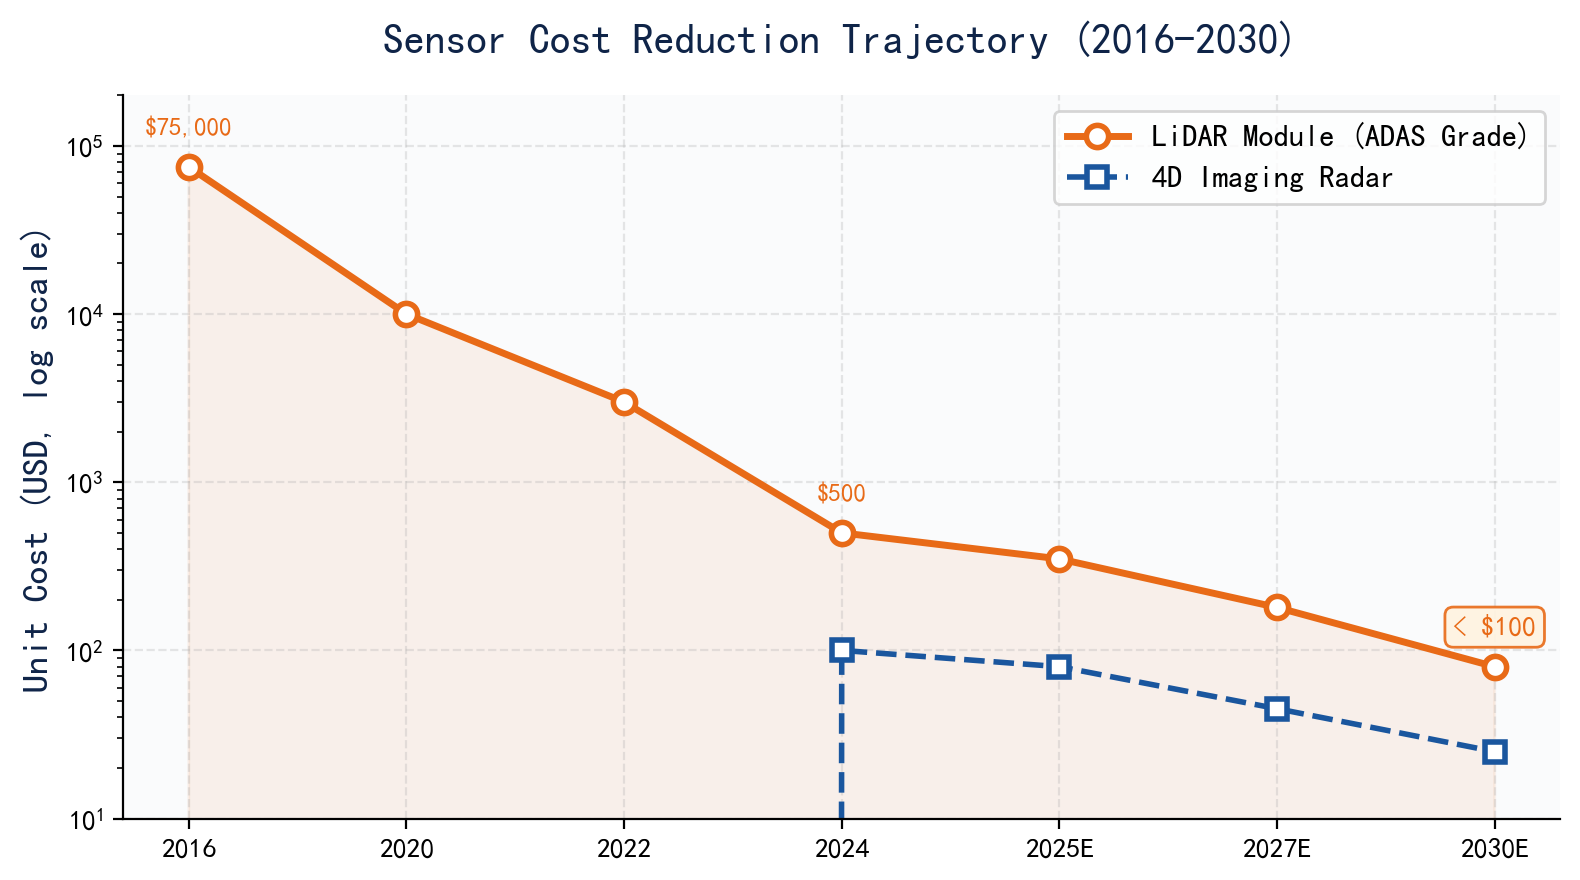
\includegraphics[width=0.85\textwidth]{figure/cost_curve.png}
\caption{自动驾驶传感器成本下降轨迹（2016-2030）}
\label{fig:cost_curve}
\end{figure}

\begin{figure}[htbp]
\centering
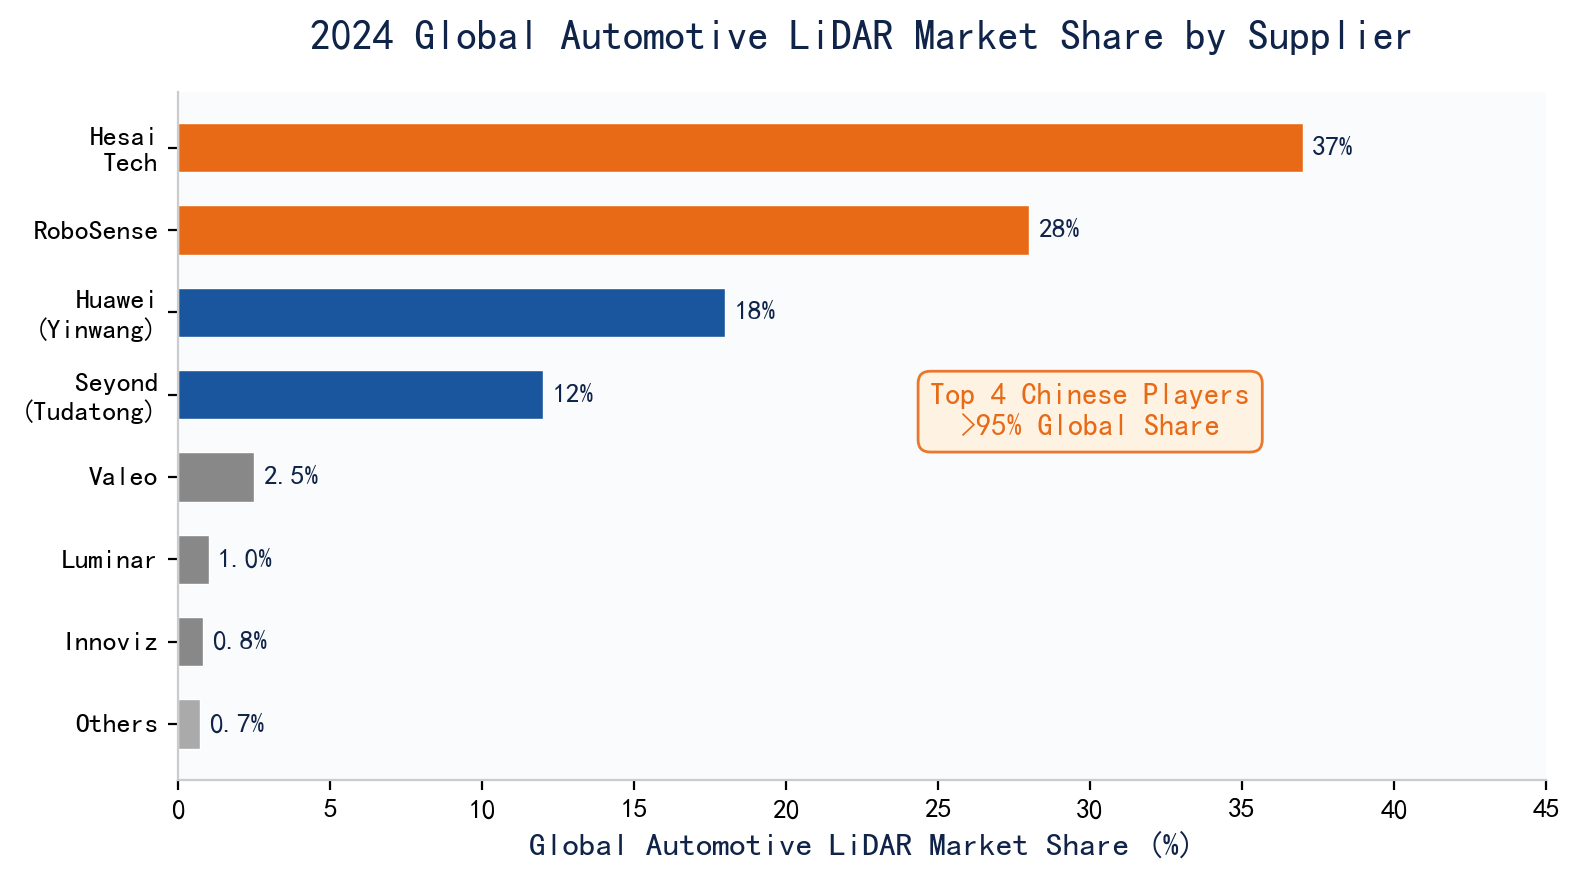
\includegraphics[width=0.85\textwidth]{figure/market_players.png}
\caption{2024年全球车载激光雷达市场份额（按供应商）}
\label{fig:market_players}
\end{figure}

\keybox{自动驾驶传感器领域当前处于严重的人才供不应求状态——供给端培养速度远落后于需求端爆发速度。对电子信息类、计算机类、自动化类毕业生而言，传感器技术与自动驾驶感知融合是当前最具成长性的细分方向之一。顶尖企业（禾赛、速腾聚创、华为车BU）对应届硕士算法岗开出25-45万年薪，资深专家级工程师年薪可达80-150万元+。}

\section{典型岗位与技能需求}

基于对禾赛科技、速腾聚创、其域创新、华为车BU、大疆车载、德赛西威等产业链核心企业的招聘信息分析，自动驾驶传感器领域的典型技术岗位及技能需求如下：

\begin{enumerate}
    \item \textbf{激光雷达硬件工程师}
    \begin{itemize}
        \item 核心技能：模拟/混合信号IC设计、光电探测器特性分析、TIA/TDC电路设计、SIP封装设计、VCSEL驱动电路
        \item 工具链：Cadence Virtuoso、ADS、HFSS、Altium Designer
        \item 知识背景：光电信息科学与工程、微电子科学与工程、电子科学与技术
    \end{itemize}

    \item \textbf{多传感器标定算法工程师}
    \begin{itemize}
        \item 核心技能：多视图几何、非线性优化（Ceres/g2o）、PnP/手眼标定、LiDAR-Camera联合标定、C++/Python
        \item 知识背景：计算机视觉、机器人学、摄影测量与遥感
    \end{itemize}

    \item \textbf{感知融合算法工程师}
    \begin{itemize}
        \item 核心技能：3D目标检测（PointPillars/CenterPoint）、BEV感知/Transformer架构、多目标跟踪（MOT/AB3DMOT）、传感器前/后融合、PyTorch/TensorRT
        \item 知识背景：计算机科学（人工智能方向）、模式识别与智能系统
    \end{itemize}

    \item \textbf{自动驾驶嵌入式系统工程师}
    \begin{itemize}
        \item 核心技能：GPGPU/CUDA编程、模型量化与TensorRT部署、QNX/Linux实时操作系统、DDS/SomeIP中间件、ROS2
        \item 知识背景：计算机体系结构、嵌入式系统、软件工程
    \end{itemize}

    \item \textbf{传感器系统集成与测试工程师}
    \begin{itemize}
        \item 核心技能：传感器性能测试（MTF、角分辨率、探测概率）、EMC/EMI测试、车规级可靠性验证（AEC-Q100/Q200）、HIL/SIL测试
        \item 知识背景：车辆工程、测控技术与仪器、电气工程
    \end{itemize}
\end{enumerate}

\section{薪资水平与发展前景}

根据2024-2025年招聘市场数据（综合猎头公司、招聘平台及企业公开薪资数据），自动驾驶传感器领域的技术岗位薪资水平（年薪，中国大陆一线城市/新一线城市，含股票/期权）大致为：

\begin{table}[htbp]
\centering
\caption{自动驾驶传感器领域典型岗位薪资区间（2024-2025年）}
\label{tab:salary}
\begin{tabular}{cccc}
\toprule
\textbf{岗位类别} & \textbf{应届硕士} & \textbf{3-5年经验} & \textbf{资深/专家（5-10年+）} \\
\midrule
感知融合算法（AI/深度学习） & 28-45万 & 50-85万 & 90-160万+ \\
标定与定位算法 & 25-40万 & 45-75万 & 80-140万+ \\
激光雷达/毫米波硬件设计 & 22-35万 & 40-65万 & 65-120万+ \\
嵌入式系统/车载软件 & 20-32万 & 35-55万 & 55-100万+ \\
系统集成与测试验证 & 15-28万 & 28-50万 & 45-85万+ \\
\bottomrule
\end{tabular}
\end{table}

\vspace{-0.5em}
\textbf{关键行业趋势：}
\begin{itemize}
    \item \textbf{人才缺口持续扩大}：中国智能网联汽车产业2025年直接人才缺口约35-50万人，其中传感器感知与算法方向占比约30\%，缺口规模约10-15万人。
    \item \textbf{薪资增速显著高于传统制造业}：自动驾驶传感器领域应届硕士薪资较传统电子信息制造业高50\%-120\%，3-5年经验后差距进一步扩大至2-3倍。
    \item \textbf{地域集中度高}：上海、深圳、北京、苏州、广州五城市集中了约80\%的自动驾驶传感器相关岗位。广深地区因比亚迪、小鹏、华为车BU、大疆车载、德赛西威、其域创新等企业的集聚效应，近年来岗位增速最为迅猛。
    \item \textbf{学历与技能门槛}：算法类岗位普遍要求硕士及以上学历（约78\%的感知算法岗位要求硕士学历）；硬件和嵌入式类岗位对硕士学历的硬性要求相对低（约40\%-55\%），但更看重项目实践经验和芯片/板级调试能力。
\end{itemize}

该领域目前处于人才供需严重失衡的状态——供给端培养速度远落后于需求端爆发速度。对电子信息类（含光电信息、微电子）、计算机类（含AI、软件工程）、自动化类（含模式识别、测控技术）专业的毕业生而言，传感器技术与自动驾驶感知融合是当前最具成长性的细分方向之一。建议在校同学通过以下路径提升竞争力：(1) 参与开源自动驾驶项目（如Apollo、Autoware）并积累真实传感器数据处理经验；(2) 在KITTI/nuScenes/Waymo Open Dataset等公开数据集上复现主流感知模型；(3) 掌握至少一种嵌入式平台的模型部署工具链（TensorRT/NCNN/ONNX Runtime）；(4) 关注目标企业（禾赛、速腾聚创、其域创新、华为车BU、大疆车载等）的实习招聘周期，提前准备。

\clearpage

% ===================== 第9章 结论 =====================
\chapter{结论与展望}

本文对自动驾驶汽车中的五类先进传感器——视觉摄像机、毫米波雷达、超声波雷达、激光雷达和惯性测量单元——从物理原理、核心元器件、测量电路到多传感器融合应用进行了系统性综述。

在物理原理层面，本文以内光电效应、电磁波FMCW信号模型、压电换能效应和牛顿惯性定律为物理基础，建立了各传感器从原始物理量到可测量电信号的完整数学模型。在核心元器件层面，从CMOS有源像素到VCSEL/SPAD光电收发对，从77GHz CMOS MMIC到MEMS振动陀螺仪，详细剖析了各器件的微观工作机制和关键技术指标。在测量电路层面，以CDS相关双采样、TIA跨阻放大器和TDC时间数字转换器为代表性案例，深入阐述了从微弱的模拟物理量到高精度数字量输出的信号调理与转换链路。

在应用与展望方面，本文指出：多传感器融合是自动驾驶感知系统不可逆转的技术方向，BEV+Transformer的前融合架构已成为产业主流范式，而GPGPU/TensorRT驱动的模型轻量化部署将深度学习感知推向了车载实时推理的边缘。市场数据表明，2025-2030年是中国自动驾驶传感器产业从"技术验证"迈向"规模化商业落地"的黄金窗口期，激光雷达和4D成像毫米波雷达是增长确定性最高的两大细分赛道。

未来，随着硅光子学、3D堆叠封装和存算一体（PIM）架构的持续推进，"传感-计算-决策"三者将在物理芯片层面实现深度融合，形成传感计算一体化的全新范式。对于有志于从事传感器技术与智能驾驶交叉领域的学生而言，扎实的物理电子学基础、电机拖动与控制理论、嵌入式系统实践与深度学习算法能力，共同构成了进入这一前沿行业的综合竞争力。

\clearpage

% ===================== 参考文献 =====================
\chapter*{\heiti 参考文献}
\addcontentsline{toc}{chapter}{参考文献}

\begin{thebibliography}{99}

\bibitem{ref1} 王庞伟等. 智能网联汽车电子技术[M]. 北京: 机械工业出版社, 2021.

\bibitem{ref2} 周润景等. 常用传感器技术及应用（第二版）[M]. 北京: 电子工业出版社, 2021.

\bibitem{ref3} 李立功等. 光电传感器原理与应用[M]. 北京: 科学出版社, 2020.

\bibitem{ref4} 程润伟等. CUDA C编程权威指南[M]. 北京: 机械工业出版社, 2017.

\bibitem{ref5} 景乃锋等. 通用图形处理器设计：GPGPU编程模型与架构原理[M]. 北京: 清华大学出版社, 2022.

\bibitem{ref6} 方吉鑫, 等. 硅光电倍增管前端放大电路的架构研究进展[J]. 激光技术, 2026, 50(2): 161-168.

\bibitem{ref7} 林远启, 等. 集成化多线列激光雷达模拟前端微组件设计[J]. 光电工程, 2021, 48(2): 210080.

\bibitem{ref8} 王伟, 张辉, 李明. 车载固态激光雷达技术发展综述[J]. 红外与激光工程, 2024, 53(1): 20230330.

\bibitem{ref9} 刘伟奇. Review of Automotive Sensors Based on Autonomous Driving[C]. IEEE Sensors, 2025.

\bibitem{ref10} Lang A H, Vora S, Caesar H, et al. PointPillars: Fast encoders for object detection from point clouds[C]//Proceedings of the IEEE/CVF Conference on Computer Vision and Pattern Recognition (CVPR). 2019: 12697-12705.

\bibitem{ref11} Li Y, Ibanez-Guzman J. Lidar for autonomous driving: The principles, challenges, and trends for automotive lidar and perception systems[J]. IEEE Signal Processing Magazine, 2020, 37(4): 50-61.

\bibitem{ref12} Behroozpour B, Sandborn P A M, Wu M C, et al. Lidar system architectures and circuits[J]. IEEE Communications Magazine, 2017, 55(10): 135-142.

\bibitem{ref13} Poulton C V, et al. Optical beamforming techniques for solid-state automotive LIDAR[R]. UC Berkeley EECS Technical Report, 2023.

\bibitem{ref14} Yole Intelligence. LiDAR for Automotive and Industrial Applications 2024[R]. Yole Group, 2024.

\bibitem{ref15} 高工智能汽车研究院. 2024年度中国乘用车前装激光雷达市场报告[R]. 2025.

\bibitem{ref16} 中商产业研究院. 2024-2029年中国激光雷达行业市场深度调研及发展前景报告[R]. 2024.

\bibitem{ref17} 中商产业研究院. 全球激光雷达市场规模报告[R]. 2024.

\bibitem{ref18} QYResearch. 全球机器人激光雷达市场预测（2023-2030）[R]. 2024.

\bibitem{ref19} 禾赛科技. AT128产品技术规格书[Z]. 2023.

\bibitem{ref20} 速腾聚创. RS-LiDAR-M1/E1平台技术白皮书[Z]. 2024.

\bibitem{ref21} 加特兰微电子. Alps系列77GHz CMOS毫米波雷达SoC数据手册[Z]. 2024.

\bibitem{ref22} 东兴证券研究所. 激光雷达产业链深度分析报告[R]. 2024.

\bibitem{ref23} 其域创新. 产品与招聘信息[EB/OL]. \url{https://xgrids.cn}. 2025.

\bibitem{ref24} 其域创新. 多传感器标定算法工程师招聘[EB/OL]. \url{https://pecivkvtit.jobs.feishu.cn/index/position/7486766416390113587/detail}. 2025.

\bibitem{ref25} 其域创新. 感知融合算法工程师招聘[EB/OL]. \url{https://pecivkvtit.jobs.feishu.cn/index/position/7491253117397387529/detail}. 2025.

\bibitem{ref26} 其域创新. 多传感器融合算法工程师(视觉雷达联合重建方向)招聘[EB/OL]. \url{https://pecivkvtit.jobs.feishu.cn/index/position/7535787737665538350/detail}. 2025.

\bibitem{ref27} IEEE Standard for Inertial Sensor Terminology. IEEE Std 528-2019[S]. 2019.

\bibitem{ref28} El-Sheimy N, Hou H, Niu X. Analysis and modeling of inertial sensors using Allan variance[J]. IEEE Transactions on Instrumentation and Measurement, 2008, 57(1): 140-149.

\bibitem{ref29} Bronzi D, Villa F, Tisa S, et al. 100 000 frames/s 64$\times$32 single-photon detector array for 2-D imaging and 3-D ranging[J]. IEEE Journal of Selected Topics in Quantum Electronics, 2014, 20(6): 354-363.

\bibitem{ref30} Pellegrini S, Rae B, Ping G A. SPAD sensors: from single photon detection to LiDAR[J]. Nature Photonics, 2022, 16: 441-448.

\bibitem{ref31} Zappa F, Tisa S, Tosi A, et al. Principles and features of single-photon avalanche diode arrays[J]. Sensors and Actuators A: Physical, 2007, 140(1): 103-112.

\bibitem{ref32} Cova S, Ghioni M, Lacaita A, et al. Avalanche photodiodes and quenching circuits for single-photon detection[J]. Applied Optics, 1996, 35(12): 1956-1976.

\bibitem{ref33} 华为技术有限公司. 华为4D成像毫米波雷达技术白皮书[Z]. 2024.

\bibitem{ref34} Continental AG. ARS540 4D Imaging Radar Technical Data Sheet[Z]. 2023.

\bibitem{ref35} 德赛西威. 自动驾驶域控制器与传感器集成方案[Z]. 2024.

\end{thebibliography}

\clearpage

% ===================== 致谢 =====================
\chapter*{\heiti 致\quad 谢}
\addcontentsline{toc}{chapter}{致谢}

感谢任课教师翟老师（zhaiyh@gdut.edu.cn）在《传感器技术与应用》课程中的系统讲授与悉心指导。课程中关于光电传感器、CCD/CMOS图像传感器、内光电效应、暗电流机理以及信号调理电路的深入讲解，为本调研报告的撰写奠定了扎实的理论基础。翟老师在授课中将理论公式推导与工程实践案例有机结合，使学生在理解传感器物理原理的同时，对实际电路设计中的性能约束与工程权衡有了直观的认知，这种\"原理-器件-电路\"三位一体的讲授方法对本文写作产生了深刻影响。

感谢广东工业大学提供的丰富的数字图书馆资源（包括IEEE Xplore、中国知网CNKI、万方数据库等），使本报告得以广泛检索和引用来自光电工程、激光技术、IEEE Signal Processing Magazine、CVPR等高水平期刊与会议的学术文献。

本报告写作过程中参考和引用了大量来自国内外激光雷达企业（禾赛科技、速腾聚创、其域创新、加特兰微电子等）、学术研究机构（UC Berkeley、MIT、清华大学、中国科学院等）以及市场研究机构（Yole Intelligence、高工智能汽车研究院、QYResearch、中商产业研究院等）的公开技术文献和市场数据。禾赛科技AT128、速腾聚创E1平台的技术文档为第五章激光雷达的器件分析提供了宝贵的一手工程资料；加特兰微电子的Alps系列芯片数据手册为第三章毫米波雷达CMOS工艺国产替代趋势的判断提供了关键依据。在此向这些推动传感器技术进步的组织和个人致以诚挚谢意。

最后，感谢家人和朋友们在调研写作期间的理解与支持。传感器的世界从微观的皮秒计时到宏观的市场千亿规模，跨度之大令人在调研中既感敬畏又觉兴奋。希望这份报告不仅能完成课程考核要求，也能为同样对自动驾驶传感器技术感兴趣的同学提供一份有参考价值的入门材料。

\clearpage

\end{document}
